%% abtex2-modelo-trabalho-academico.tex, v-1.9.6 laurocesar
%% Copyright 2012-2016 by abnTeX2 group at http://www.abntex.net.br/ 
%%
%% This work may be distributed and/or modified under the
%% conditions of the LaTeX Project Public License, either version 1.3
%% of this license or (at your option) any later version.
%% The latest version of this license is in
%%   http://www.latex-project.org/lppl.txt
%% and version 1.3 or later is part of all distributions of LaTeX
%% version 2005/12/01 or later.
%%
%% This work has the LPPL maintenance status `maintained'.
%% 
%% The Current Maintainer of this work is the abnTeX2 team, led
%% by Lauro César Araujo. Further information are available on 
%% http://www.abntex.net.br/
%%
%% This work consists of the files abntex2-modelo-trabalho-academico.tex,
%% abntex2-modelo-include-comandos and abntex2-modelo-references.bib
%%

% ------------------------------------------------------------------------
% ------------------------------------------------------------------------
% abnTeX2: Modelo de Trabalho Academico (tese de doutorado, dissertacao de
% mestrado e trabalhos monograficos em geral) em conformidade com 
% ABNT NBR 14724:2011: Informacao e documentacao - Trabalhos academicos -
% Apresentacao
% ------------------------------------------------------------------------
% ------------------------------------------------------------------------


\documentclass[
  10.5pt,				  % tamanho da fonte
	openright,			% capítulos começam em pág ímpar (insere página vazia caso preciso)
	twoside,			  % para impressão em recto e verso. Oposto a oneside  
  a5paper,
  chapter=TITLE,	% títulos de capítulos convertidos em letras maiúsculas
	section=TITLE,	% títulos de seções convertidos em letras maiúsculas
  hyphens,        % faz a quebra de linhas em URLs muito longas
	% -- opções do pacote babel --
	english,        % idioma adicional para hifenização
	brazil          % o último idioma é o principal do documento
]{abntex2}

% ---
% Pacotes básicos 
% ---
\usepackage{lmodern}          % Usa a fonte Latin Modern			
\usepackage[T1]{fontenc}      % Selecao de codigos de fonte.
\usepackage[utf8]{inputenc}	  % Codificacao do documento (conversão automática dos acentos)
\usepackage{lastpage}         % Usado pela Ficha catalográfica
\usepackage{indentfirst}      % Indenta o primeiro parágrafo de cada seção.
\usepackage{color}				    % Controle das cores
\usepackage{graphicx}			    % Inclusão de gráficos
\usepackage{microtype} 			  % Para melhorias de justificação
\usepackage[final]{pdfpages}
\usepackage{listings}         % Para incluir código fonte com formatação
\usepackage{lscape}           % Folha em formato landscape

\usepackage{multirow}         % Permite a mesclagem de linhas em tabelas
\usepackage[normalem]{ulem}   % Permite riscar palavras
\usepackage{enumitem}         % Permite renomear os itens de itemize
%\usepackage{adjustbox}        % Permite o escalonamento do conteúdo que não cabe em uma página
%\usepackage{tabularx}         % Impede o overflow de tabelas. 
%\usepackage{rotating}         % Rotaciona tabelas.
%\usepackage{placeins}         % Permite usar \FloatBarrier

% ---

% ---
% Pacotes adicionais, usados apenas no âmbito do Modelo Canônico do abnteX2
% ---
\usepackage{lipsum}				% para geração de dummy text
%\usepackage{cmap}
% ---

% ---
% Lista de símbolos e acrônimos
% ---
%\usepackage{abntex2glossaries}  % Deve ser incluído antes de abntex2cite

% ---
% Pacotes de citações
% ---
\usepackage[brazilian,hyperpageref]{backref} % Paginas com as citações na bibl
\usepackage[alf]{abntex2cite}	               % Citações utilizando o padrão autor-data de chamadas
%\usepackage[num,overcite]{abntex2cite}       % Citações utilizando o padrão numérico de chamadas
\citebrackets()


% --- 
% CONFIGURAÇÕES DE PACOTES
% --- 

% ---
% Configurações do pacote backref
% Usado sem a opção hyperpageref de backref
\renewcommand{\backrefpagesname}{Citado na(s) página(s):~}
% Texto padrão antes do número das páginas
\renewcommand{\backref}{}
% Define os textos da citação
\renewcommand*{\backrefalt}[4]{
	\ifcase #1 %
		Nenhuma citação no texto.%
	\or
		Citado na página #2.%
	\else
		Citado #1 vezes nas páginas #2.%
	\fi}%
% ---

% ---
% Correção das margens
% ---
\setlrmarginsandblock{2.5cm}{1.5cm}{*}
\setulmarginsandblock{2.0cm}{1.5cm}{*}
\checkandfixthelayout
% ---
% Correção das fontes das seções
% ---
%\renewcommand{\ABNTEXchapterfont}{\fontfamily{lm}\fontseries{b}\selectfont}
\renewcommand{\ABNTEXchapterfont}{\fontfamily{cmr}\fontseries{b}\selectfont}
\renewcommand{\ABNTEXchapterfontsize}{\normalsize}
\renewcommand{\ABNTEXsectionfont}{\ABNTEXchapterfont}
\renewcommand{\ABNTEXsectionfontsize}{\normalsize}
\renewcommand{\ABNTEXsubsectionfont}{\ABNTEXchapterfont}
\renewcommand{\ABNTEXsubsectionfontsize}{\normalsize}
\renewcommand{\ABNTEXsubsubsectionfont}{\ABNTEXchapterfont}
\renewcommand{\ABNTEXsubsubsectionfontsize}{\normalsize}
% ---
% Correção do espaçamento no primeiro parágrafo
% ---
\setlength\afterchapskip{\lineskip}
% ---
% Caminho para as imagens
% ---
\graphicspath{{./img/}}
% ---
% Listings
% ---
\renewcommand{\lstlistingname}{Algoritmo}% Listing -> Algoritmo
\renewcommand{\lstlistlistingname}{Lista de \lstlistingname s}% List of Listings -> Lista de Algoritmos
\definecolor{mygreen}{rgb}{0,0.6,0}
\definecolor{mygray}{rgb}{0.5,0.5,0.5}
\definecolor{mymauve}{rgb}{0.58,0,0.82}
\lstset{ %
  backgroundcolor=\color{white},     % choose the background color;
  basicstyle=\footnotesize\ttfamily, % the size of the fonts that are used for the code
  breakatwhitespace=false,           % sets if automatic breaks should only happen at whitespace
  breaklines=true,                 % sets automatic line breaking
  captionpos=t,                    % sets the caption-position to bottom
  commentstyle=\color{mygreen},    % comment style
  deletekeywords={...},            % if you want to delete keywords from the given language
  escapeinside={\%*}{*)},          % if you want to add LaTeX within your code
  extendedchars=true,              % lets you use non-ASCII characters; for 8-bits encodings only, does not work with UTF-8
  frame=single,	                   % adds a frame around the code
  keepspaces=true,                 % keeps spaces in text, useful for keeping indentation of code (possibly needs columns=flexible)
  keywordstyle=\color{blue},       % keyword style
  language=Java,                   % the language of the code
  morekeywords={*,...},            % if you want to add more keywords to the set
  numbers=none,                    % where to put the line-numbers; possible values are (none, left, right)
  numbersep=5pt,                   % how far the line-numbers are from the code
  numberstyle=\tiny\color{mygray}, % the style that is used for the line-numbers
  rulecolor=\color{black},         % if not set, the frame-color may be changed on line-breaks within not-black text (e.g. comments (green here))
  showspaces=false,                % show spaces everywhere adding particular underscores; it overrides 'showstringspaces'
  showstringspaces=false,          % underline spaces within strings only
  showtabs=false,                  % show tabs within strings adding particular underscores
  stepnumber=2,                    % the step between two line-numbers. If it's 1, each line will be numbered
  stringstyle=\color{mymauve},     % string literal style
  tabsize=2,	                     % sets default tabsize to 2 spaces
  title=\lstname,                  % show the filename of files included with \lstinputlisting; also try caption instead of title
  numberbychapter=false            % number lists by chapter or sequentially from the beginning of the document
}

% ----------------------------------------------------------
% PREÂMBULO
% ----------------------------------------------------------

\titulo{Atualização Tecnológica do Formulário de Inscrição do Processo Seletivo da Pós-Graduação da UFSC}
\autor{Makhles Reuter Lange}
\data{\today}
%\instituicao{Universidade Federal de Santa Catarina}
\instituicao{%
  Universidade Federal de Santa Catarina - UFSC
  \par
  Ciências da Computação}
\local{Florianópolis}
\tipotrabalho{Exemplo para referência futura}
\orientador{Andréia Alves dos Santos Schwaab}
\coorientador{Leandro José Komosinski}
\tipotrabalho{Trabalho de Conclusão de Curso}
\preambulo{Relatório Final do Trabalho de Conclusão dc Curso do Curso de Ciências da Computação da Universidade Federal de Santa Catarina.}
%TODO
%\preambulo{Trabalho de Conclusão de Curso submetido ao Curso de Ciências da Computação da Universidade Federal de Santa Catarina para a obtenção do grau de Bacharel em Ciências da Computação.}

% ---
% Configurações de aparência do PDF final

% alterando o aspecto da cor azul
\definecolor{blue}{RGB}{41,5,195}

% informações do PDF
\makeatletter
\hypersetup{
     	%pagebackref=true,
		pdftitle={\@title}, 
		pdfauthor={\@author},
    	pdfsubject={\imprimirpreambulo},
	    pdfcreator={TeXmaker},
		pdfkeywords={tcc}{latex}{primefaces}{java}{jsf}{trabalho acadêmico}, 
		colorlinks=true,       		% false: boxed links; true: colored links
    	linkcolor=blue,          	% color of internal links
    	citecolor=blue,        		% color of links to bibliography
    	filecolor=magenta,      		% color of file links
		urlcolor=blue,
		bookmarksdepth=4
}
\makeatother
% --- 

% --- 
% Espaçamentos entre linhas e parágrafos 
% --- 

% O tamanho do parágrafo é dado por:
\setlength{\parindent}{1.0cm}

% Controle do espaçamento entre um parágrafo e outro:
\setlength{\parskip}{0.2cm}  % tente também \onelineskip

\begin{document}

% Seleciona o idioma do documento (conforme pacotes do babel)
\selectlanguage{brazil}

% Retira espaço extra obsoleto entre as frases.
\frenchspacing


% ----------------------------------------------------------
% ELEMENTOS PRÉ-TEXTUAIS
% ----------------------------------------------------------
\pretextual%
% ---
% Capa
% ---
\imprimircapa%
% ---
% Folha de rosto
% (o * indica que haverá a ficha bibliográfica)
% ---
\imprimirfolhaderosto*%
% ---
\clearpage
%\imprimirfichacatalografica%
%\clearpage

% ----------------------------------------------------------
% FOLHA DE APROVAÇÃO
% ----------------------------------------------------------

% Isto é um exemplo de Folha de aprovação, elemento obrigatório da NBR
% 14724/2011 (seção 4.2.1.3). Você pode utilizar este modelo até a aprovação
% do trabalho. Após isso, substitua todo o conteúdo deste arquivo por uma
% imagem da página assinada pela banca com o comando abaixo:
%
%\includepdf{folhadeaprovacaoassinada.pdf}
%
%TODO 
%\begin{folhadeaprovacao}
%
%  \begin{center}
%    {\ABNTEXchapterfont\large\imprimirautor}
%
%    \vspace*{\fill}\vspace*{\fill}
%    \begin{center}
%      \ABNTEXchapterfont\bfseries\Large\imprimirtitulo
%    \end{center}
%    \vspace*{\fill}
%    
%    \hspace{.45\textwidth}
%    \begin{minipage}{.5\textwidth}
%        \imprimirpreambulo
%    \end{minipage}%
%    \vspace*{\fill}
%   \end{center}
%        
%   Trabalho aprovado. \imprimirlocal, \imprimirdata:
%
%   \assinatura{\textbf{\imprimirorientador} \\ Orientador} 
%   \assinatura{\textbf{\imprimircoorientador} \\ Coorientador}
%   \assinatura{\textbf{Beatriz Wilges} \\ Convidado 1}
%   \assinatura{\textbf{Verônica de Souza de Melo} \\ Convidado 2}
%
%   \begin{comment}
%  \begin{center}
%    \vspace*{0.5cm}
%    {\large\imprimirlocal}
%    \par
%    {\large\imprimirdata}
%    \vspace*{1cm}
%  \end{center}
%  \end{comment}
%\end{folhadeaprovacao}


% ----------------------------------------------------------
% RESUMOS
% ----------------------------------------------------------
 
\begin{resumo}

Utilizando-se a linguagem Java e as tecnologias para desenvolvimento Web próprias do JavaEE, desenvolveu-se um sistema de inscrição para os Programas de Pós-Graduação da UFSC. A produção deste trabalho foi inspirada em um sistema atualmente em uso que está carente de algumas funcionalidades. O novo sistema permite o prenchimento do formulário durante todo o período definido no cronograma do processo seletivo, além do envio de documentos obrigatórios pré-estabelecidos pelas secretarias dos cursos e da importação dos dados de inscrições passadas. A interface do sistema foi desenvolvida de forma responsiva, \emph{i.e.}, a usabilidade em dispositivos móveis também foi levada em consideração no desenvolvimento das páginas. Ainda, empregou-se um conjunto de bibliotecas mais atual do que o do sistema em uso, proporcionando mais recursos ao desenvolvedor. Atualmente o sistema se encontra no estágio de homologação e à espera de testes e identificação de possíveis \emph{bugs} e melhorias.

\vspace{\onelineskip}
\noindent \textbf{Palavras-chave:} Formulário de Inscrição; Processo Seletivo; Desenvolvimento Web; JavaServer Faces; PrimeFaces; Responsive Web Design.
\end{resumo}
%% ---
\begin{resumo}[Abstract]
\begin{otherlanguage*}{english}

JavaEE Web development technologies were used in the development of a new online Postgraduate Enrollment System for the Federal University of Santa Catarina. The current enrollment system, which lacks some important sought out functionalities, was used as an inspiration in the development of the new one. Candidates can now fill out the application forms at any time during the selection process, upload the required documents and import personal data used in the last submitted application. Responsive web design was taken into consideration while designing the system, \emph{i.e.}, mobile users will not feel left behind when filling out the application form. Lastly, an up-to-date set of libraries were used instead of the old ones, providing a more resourceful environment to developers. The system is currently awaiting tests and improvements.

\vspace{\onelineskip}
\noindent \textbf{Keywords:} Application Form; Selection Process; Web Development; JavaServer Faces; PrimeFaces; Responsive Web Design.
\end{otherlanguage*}
\end{resumo}


% ---
% Lista de ilustrações
% ---
\pdfbookmark[0]{\listfigurename}{lof}
\listoffigures*
\cleardoublepage
% ---

% ---
% Lista de tabelas
% ---
\pdfbookmark[0]{\listtablename}{lot}
\listoftables*
\cleardoublepage
% ---

% ---
% Lista de abreviaturas e siglas
% ---
\begin{siglas}
  \item[CAS]     Sistema de Autenticação Centralizada
  \item[Java EE] Java Enterprise Edition
  \item[JSF]     JavaServer Faces
  \item[JPA]     Java Persistence API
  \item[PROPG]   Pró-Reitoria de Pós-Gradução
  \item[RUP]     Rational Unified Process
  \item[SeTIC]   Superintendência de Governança Eletrônica e Tecnologia da Informação e Comunicação
  \item[UFSC]    Universidade Federal de Santa Catarina
  \item[UML]     Unified Modelling Language
\end{siglas}



% ----------------------------------------------------------
% SUMÁRIO
% ----------------------------------------------------------
\pdfbookmark[0]{\contentsname}{toc}
\tableofcontents*
\cleardoublepage
% ---



% ----------------------------------------------------------
% ELEMENTOS TEXTUAIS
% ----------------------------------------------------------
\textual%


\pagenumbering{arabic}
\setcounter{page}{5}

\chapter{Introdução}
% ----------------------------------------------------------

% ---
\section{Contextualização}
% ---

O acesso aos programas de pós-graduação oferecidos pela Universidade Federal de Santa Catarina é feito através de processos seletivos lançados por suas respectivas secretarias. Todos os programas possuem algum modo para realizar as inscrições em seus processos seletivos. Dentre as formas utilizadas, destacam-se um sistema informatizado oficial, formulários de inscrição manuais e sistemas informatizados não-oficiais.
O uso desses diversos sistemas, com suas funcionalidades e interfaces distintas, acarreta em diversos problemas, tais como:
\begin{itemize}
  \item Falta de padronização dos requisitos e tecnologias utilizadas.
  \item Autenticação de forma não-centralizada: além de ser uma vulnerabilidade em termos de segurança, implica em duplicação de código.
  \item Difícil manutenibilidade;
  \item Difícil obtenção de estatísticas relacionadas aos candidatos.
\end{itemize}

Em meados de 2010, esperava-se mais de cinco mil inscrições no Programa de Especialização em Saúde da Família. Visando atender essas inscrições, a solução adotada pela Pró-Reitoria de Pós-Gradução (PROPG), em parceria com a Superintendência de Governança Eletrônica e Tecnologia da Informação e Comunicação (SeTIC), foi a criação de um sistema informatizado\footnote{Vide \href{http://www.capg.ufsc.br/inscricao}{http://www.capg.ufsc.br/inscricao}}. Posteriormente, esse sistema foi adotado por outros programas.

A Figura~\ref{fig:uso_sistemas} mostra o uso desse sistema pelos programas da UFSC em 2017. Dos 113 programas, apenas 67 (59\%) adotaram o sistema para realizar as inscrições. A figura também mostra o uso de acordo com o tipo do programa (\emph{stricto sensu} ou \emph{lato sensu}).


\begin{figure}[!ht]
  \caption{\label{fig:uso_sistemas}Utilização dos sistemas de inscrição em 2017.}
  \begin{center}
    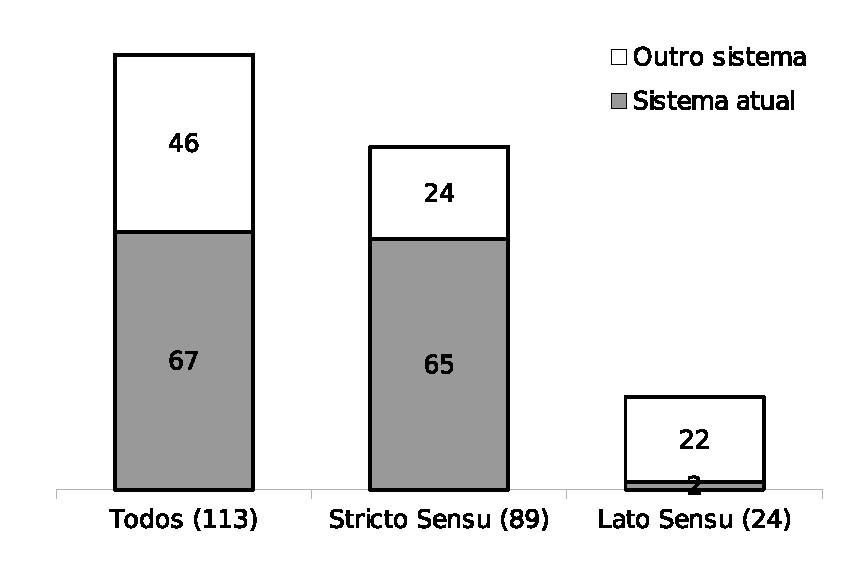
\includegraphics[width=0.75\textwidth]{uso_sistema_atual}
  \end{center}
  \fonte{Dados obtidos em consultas ao banco de dados do CAPG.}
\end{figure}

Não obstante, esse sistema não foi desenvolvido visando a integração dos sistemas existentes e está carente de algumas funcionalidades frequentemente solicitadas pelos programas de pós-graduação. A implementação de tais funcionalidades no sistema atual é custosa, pois sua estrutura contempla os requisitos definidos na época de sua elaboração. Adicionalmente, as bibliotecas e tecnologias utilizadas são antigas\footnote{Algumas estão, inclusive, descontinuadas.}, dificultando seu desenvolvimento e sua manutenibilidade. Justifica-se, portanto, o desenvolvimento de um novo sistema de inscrição, que terá como inspiração o sistema atual, porém com a atualização das tecnologias utilizadas e a adição das funcionalidades descritas nas seções~\ref{sec:envio_doc}~e~\ref{sec:ordem}.

\subsection{Envio de documentos}\label{sec:envio_doc}
A funcionalidade mais importante que será implementada neste novo sistema é o envio de documentos de forma digital por parte dos candidatos, que atualmente têm o trabalho de comparecer às secretarias dos cursos com as cópias físicas dos documentos. A praticidade dessa funcionalidade beneficia tanto o candidato quanto a universidade.

\subsection{Salvamento progressivo das informações}
Caso um candidato queira fazer a inscrição em algum dos programas de Pós-Graduação da UFSC através do sistema de inscrição atualmente em uso, este deve, essencialmente, fornecer todas as informações em uma única sessão. Ao final, o sistema fornece um número de inscrição e a possibilidade de impressão de um comprovante de inscrição.

Pretende-se oferecer ao candidato a opção de salvar o progresso do preenchimento do formulário. O candidato poderá, dessa forma, distribuir o preenchimento do formulário em várias sessões até que esteja seguro das informações fornecidas e decida-se por finalizar sua inscrição.

\subsection{Ordem de preenchimento do formulário}\label{sec:ordem}
No sistema atual, o preenchimento do formulário segue uma ordem predefinida. Muitas vezes, no entanto, o candidato não possui todas as informações necessárias e/ou relevantes ao iniciar o preenchimento do formulário. Pretende-se dar a possibilidade de preenchimento do formulário sem nenhuma ordem imposta neste processo\footnote{A não ser em situações onde exista uma ordem implícita. O envio de documentos é um exemplo, pois estes dependem do programa e nível escolhidos.}.

% ---
\section{SeTIC}
% ---

A Superintendência de Governança Eletrônica e Tecnologia da Informação e Comunicação (SeTIC), setor de informática da Universidade Federal de Santa Catarina (UFSC), é responsável pelo planejamento, pesquisa, aplicação e desenvolvimento de produtos e serviços de tecnologia da informação e comunicação da universidade\footnote{Mais informações em http://setic.ufsc.br/apresentacao/}. As aplicações desenvolvidas pela SeTIC são solicitadas e acompanhadas por usuários dos diversos setores da UFSC.

Ressalta-se que o autor deste trabalho já foi estagiário na SeTIC e que, durante o período de desenvolvimento deste, teve bolsa de extensão fornecida pela FEESC. Todas as atividades foram desenvolvidas nas instalações da SeTIC, com equipamentos e tecnologias disponibilizados por esta. Assim, o último estágio do desenvolvimento do presente sistema, \emph{i.e.}, a \emph{operacionalização} e a \emph{manutenção}\footnote{O sistema é liberado e implantado no ambiente de produção. Eventuais erros que não foram descobertos nos estágios anteriores e novos requisitos podem surgir ao longo do uso do sistema, justificando a sua constante manutenção.}, serão feitas pela SeTIC.

% ---
\section{Objetivos}
% ---

% ---
\subsection{Objetivo Geral}
% ---
O objetivo principal deste Trabalho de Conclusão de Curso é desenvolver um novo sistema informatizado para a inscrição de candidatos nos processos seletivos dos diversos programas de Pós-Graduação da UFSC, tendo como inspiração o sistema de inscrição que está em uso atualmente.

% ---
\subsection{Objetivos Específicos}
% ---
\begin{itemize}
  \item Implementar as \emph{regras de negócio} da inscrição em um processo seletivo, \emph{i.e.}, o \emph{back-end} da aplicação.
  \item Criar as tabelas necessárias no banco de dados.
  \item Implementar a interface com o usuário, \emph{i.e.}, as páginas que o candidato terá acesso ao realizar sua inscrição.
  \item Tornar o sistema acessível em dispositivos móveis.
  \item Disponibilizar o sistema em ambiente de homologação.
  \item Elaborar um artigo referente ao TCC.
\end{itemize}

% --- 
\section{Resultados Esperados}
% ---
\begin{itemize}
  \item Sistema CAPG Inscrição publicado no ambiente de homologação.
  \item Artigo referente à produção realizada anexo ao TCC.
\end{itemize}



\chapter{Fundamentação Teórica}
% ----------------------------------------------------------

% ---
%\section{Aplicações Web}
% ---


% ---
\section{Plataforma Java, Edição Empresarial}\label{sec:java2e}
% ---

As \textbf{aplicações empresariais} têm o propósito de fornecer a \emph{lógica do negócio} de uma empresa. O seu gerenciamento é feito de forma centralizada e é comum a sua interação com outros softwares empresariais. A plataforma Java, Edição Empresarial (Java EE), é um conjunto de tecnologias Java que são utilizadas para o desenvolvimento de aplicações empresariais. O objetivo da plataforma é fornecer aos desenvolvedores um conjunto de especificações / APIs que permitam a diminuição do tempo de desenvolvimento, a redução da complexidade e o aumento do desempenho de aplicações empresariais \cite{javaee7}. Tais especificações são \emph{contratos} que são implementados por diversos fornecedores, \emph{e.g.}, GlassFish, Oracle WebLogic, Apache TomEE, etc.

% ---
\subsection{Aplicações Multi-Camadas}
% ---

Segundo o modelo Java EE, as aplicações são distribuídas em camadas (\emph{tiered design})\footnote{Os termos \emph{tier} e \emph{layer} são ambos traduzidos para o português como ``camada''. No entanto, uma \emph{tier} representa uma unidade física, na qual um código ou processo é executado. Uma \emph{layer}, por sua vez, representa uma unidade lógica, responsável pela organização lógica do código através da abstração dos dados. Diversas \emph{layers} podem existir em computadores diferentes, ou em processos diferentes em um único computador, ou ainda em um único processo em um único computador \cite{lhotka}.}. Define-se, desta forma, responsabilidades distintas para as diferentes partes do sistema, \emph{i.e.}, para os diferentes componentes que compõem uma aplicação Java EE (vide Figura~\ref{fig:multitiered_app}) e que são distribuídos nas camadas Cliente, Web, Negócio e EIS.

\begin{figure}[!ht]
  \caption{\label{fig:multitiered_app}Componentes Java EE distribuídos nas diversas camadas de duas aplicações Web.}
  \begin{center}
    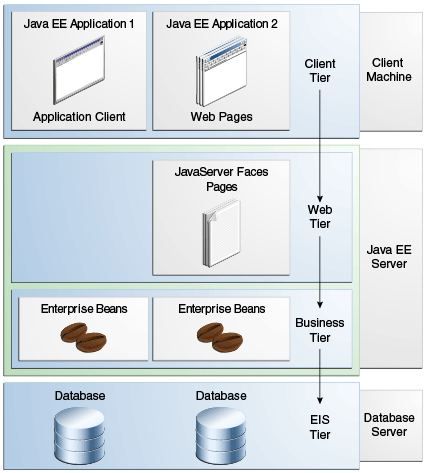
\includegraphics[width=0.75\textwidth]{multitiered_applications.png}
  \end{center}
  \fonte{adaptado de \citetext{javaee7}}
\end{figure}

% ---
\subsubsection{Camada Cliente}
% ---

Esta camada é composta de clientes aplicativos que acessam o servidor Java EE e que geralmente se localizam em máquinas diferentes da máquina do servidor:

\begin{itemize}
  \item Clientes Web - também chamados de \emph{clientes magros}, são compostos de páginas dinâmicas (\emph{e.g.}, XHTML) geradas na camada Web e por um navegador responsável por renderizá-las.
  \item Clientes Aplicativos - quando os usuários necessitam realizar atividades que requerem uma interface mais rica do que a disponibilizada por linguagens de marcação, utilizam-se clientes aplicativos baseados nas APIs Swing ou AWT (\emph{Abstract Window Toolkit}). Não obstante, pode-se utilizar uma interface em linha de comando. Embora seja possível o estabelecimento de uma conexão HTTP com um \emph{servlet} na camada Web, clientes aplicativos costumam acessar diretamente os \emph{beans} gerenciais da camada de negócio.
  \item \emph{Applets} - componentes embarcados que são incluídos nas páginas web. São escritos em Java e, portanto, necessitam da máquina virtual Java instalada no navegador web do cliente (e provavelmente do \emph{plugin} Java e de um arquivo de política de segurança).
\end{itemize}

% ---
\subsubsection{Camada Web}\label{sec:camada-web}
% ---

É a camada responsável pela interação entre os clientes e a camada de negócios. Suas principais funções são:
\begin{itemize}
  \item Gerar, dinamicamente, conteúdo para o cliente em diversos formatos.
  \item Obter as entradas (dados e ações) da interface com o cliente e retornar os resultados dos componentes da camada de negócios.
  \item Controlar o fluxo das páginas no cliente.
  \item Manter o estado dos dados da sessão do usuário.
  \item Executar um pouco de lógica simples e armazenar dados em componentes JavaBeans temporariamente.
\end{itemize}

\emph{Servlets} (vide Anexo~\ref{anexo:servlets}) e páginas web criadas com a tecnologia \emph{JavaServer Faces} (vide seção~\ref{sec:jsf}) são os componentes desta camada. 


% ---
\subsubsection{Camada de Negócio}\label{sec:camada-negocio}
% ---
A camada de negócios possui componentes que provêm a lógica do negócio da aplicação, ou seja, código que provê funcionalidades para um determinado domínio do negócio. As tecnologias utilizadas nessa camada são as seguintes:
\begin{itemize}
  \item Componentes Enterprise JavaBeans (EJB), que fornecem funcionalidades como gerenciamento de sessão, segurança, gerenciamento de transações, etc.
  \item \emph{Web services} (JAX-RS, JAX-WS).
  \item Java Persistence API (JPA), para a criação e gerenciamento de entidades (vide Seção~\ref{sec:jpa}).
\end{itemize}


% ---
\subsubsection{Camada EIS}
% ---

A camada EIS consiste de servidores de bancos de dados, sistemas de planejamento de recursos empresariais e outras fontes de dados legados. Esses recursos geralmente se localizam em suas próprias máquinas e são acessados pela camada de negócios. As tecnologias utilizadas nessa camada são:
\begin{itemize}
  \item Java Database Connetivity API (JDBC) - uma interface que permite a conexão às bases de dados.
  \item Java Persistence API (JPA).
  \item Java Transaction API (JTA) - uma interface para a realização de transações.
\end{itemize}

% ---
\subsection{JavaServer Faces}\label{sec:jsf}
% ---

A tecnologia JavaServer Faces (JSF) é uma \emph{especificação} de uma API Java utilizada para a criação de interfaces de usuário em aplicações web. Com essa API, é possível:
%
\begin{itemize}
  \item Representar componentes\footnote{Componentes, ou \emph{widgets}, são entidades autônomas e reutilizáveis da interface de usuário.} e gerenciar seus estados;
  \item Fazer o controle de eventos gerados;
  \item Realizar a validação e a conversão de dados no lado do servidor;
  \item Definir regras para a navegação entre páginas;
  \item Prover o suporte à internacionalização e acessibilidade;
\end{itemize}
%

Existem diversas implementações da especificação --- Apache MyFaces e Oracle Mojarra são as principais. Ambas contêm pelo menos os componentes padrões, ou seja, os componentes responsáveis por gerar qualquer um dos elementos HTML básicos (tabelas, caixas de entrada de texto, botões, seletores, etc). Bibliotecas de componentes podem ser utilizadas como suporte às implementações (vide Seção~\ref{sec:primefaces}).


\subsubsection{Arquitetura do \emph{Framework}}

O \emph{framework} JSF segue o padrão arquitetural\footnote{Um padrão arquitetural expressa um esquema de organização estrutural para sistemas baseados em \emph{software}. O padrão provê um conjunto de subsistemas predefinidos, especifica suas responsabilidades, e inclui regras e diretrizes para organizar a relação entre eles \cite{buschmann96}.} MVC baseado em componentes. A grande vantagem do padrão MVC é a separação entre apresentação e comportamento (lógica) da aplicação:

\begin{itemize}
  \item \textbf{M}odelo - representa o comportamento da aplicação em termos do domínio do problema.
  \item \textbf{V}isão - fornece a representação da informação para o usuário da aplicação. Pode-se ter diversas visões do mesmo modelo. A tecnologia padrão utilizada pelo JSF é a Facelets (vide Seção~\ref{sec:facelets}).
  \item \textbf{C}ontrolador - converte entradas/eventos em comandos para a visão ou para o modelo.
\end{itemize}

Os \emph{frameworks} MVC podem ser baseados em ações (\emph{action-based}) ou em componentes (\emph{component-based}). Em ambos os tipos, todas as requisições feitas à aplicação devem passar primeiramente por um controlador frontal, como pode ser visto nas Figuras~\ref{fig:mvc-push}~e~\ref{fig:mvc-pull}.

Quando se utiliza um \emph{framework} baseado em ação (\emph{e.g.}, SpringMVC, Struts, ASP.NET, etc), o controlador frontal é um \emph{servlet} que irá lidar com objetos \texttt{HTTPServletRequest} e \texttt{HTTPServletResponse}, e delegar as requisições para métodos de outros controladores (classes que estendem a classe \texttt{HttpServlet} - vide o Algoritmo~\ref{alg:servlet}, no Anexo~\ref{anexo:servlets}) de acordo com o caminho do recurso desejado e dos parâmetros da requisição. A obtenção, conversão e validação dos parâmetros das requisições e a atualização dos valores do modelo são responsabilidades do desenvolvedor da aplicação.

\begin{figure}[!ht]
  \caption{\label{fig:mvc-push}\emph{Framework} MVC baseado em ações. Os números ao lado das setas indicam a ordem do processamento de uma requisição.}
  \begin{center}
    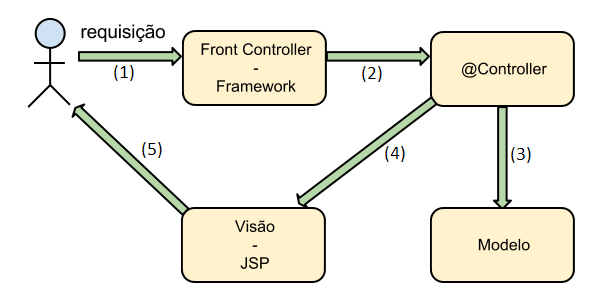
\includegraphics[width=0.75\textwidth]{/mvc/action-based.png}
  \end{center}
  \fonte{Caelum. Adaptado de \citetext{caelum}}
\end{figure}

O JSF é um \emph{framework} baseado em componentes. Como tal, possui um controlador frontal, o \texttt{FacesServlet}, que é o \emph{servlet} responsável por gerenciar o ciclo de vida do processamento de requisições. Dessa forma, o desenvolvedor da aplicação não precisa se preocupar em escrever código \emph{boilerplate}\footnote{Trechos de código que são incluídos em diversos lugares com um mínimo de alteração.}, tal como no caso de um framework baseado em ações.

Resumidamente, a requisição feita pelo usuário da aplicação é recebida pelo \texttt{FacesServlet}, que delega o processamento para a visão responsável pela geração da página acessada. O componente acessado (por exemplo, um botão) invoca um método em um \emph{managed bean}\footnote{Uma classe Java que trabalha junto à visão.}. Este, por sua vez, pode buscar dados do modelo e retorná-los para a visão. Finalmente, a visão envia a resposta ao usuário.

\begin{figure}[!ht]
  \caption{\label{fig:mvc-pull}\emph{Framework} MVC baseado em componentes. Os números ao lado das setas indicam a ordem do processamento de uma requisição.}
  \begin{center}
    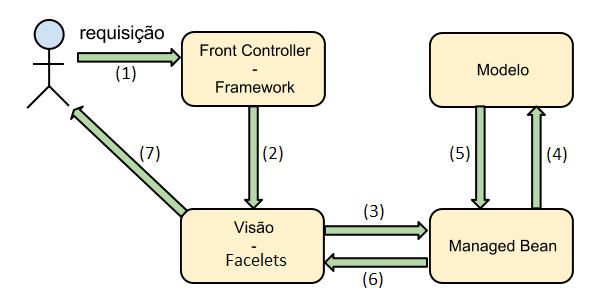
\includegraphics[width=0.75\textwidth]{/mvc/component-based.png}
  \end{center}
  \fonte{Caelum. Adaptado de \citetext{caelum}}
\end{figure}

O ciclo de vida do processamento de requisições do JSF é, na verdade, bem mais complexo do que o apresentado, pois envolve a criação de uma árvore de componentes, a conversão e validação dos dados obtidos destes componentes, o gerenciamento de eventos oriundos destes componentes e a propagação dos dados para os \emph{beans}.



% ---
\subsection{Facelets}\label{sec:facelets}
% ---
\emph{Facelets} é uma tecnologia de apresentação utilizada em aplicações baseadas em JSF. Atualmente, é também a tecnologia definida na especificação do JSF, substituindo assim a descontinuada JSP (JavaServer Pages).

Com esta tecnologia, as páginas web são criadas em XHTML e os componentes são inseridos através de \emph{tags} de diversas bibliotecas. No Algoritmo~\ref{alg:tags}, por exemplo, utiliza-se o componente \texttt{<h:inputText>}, da biblioteca JSF HTML, para a entrada de texto, e \texttt{<f:validateLongRange>}, da biblioteca Core, para a validação do texto entre um valor mínimo e um máximo.

\begin{lstlisting}[language=html, caption={Utilização de \emph{tags} em um arquivo XHTML.}, label={alg:tags}]
<html xmlns="http://www.w3.org/1999/xhtml"
      xmlns:h="http://xmlns.jcp.org/jsf/html"
      xmlns:f="http://xmlns.jcp.org/jsf/core">

<h:body>
  <h:form>
    <h:inputText id="userNumber"
                 title="Insira um numero entre 0 e 10:"
                 value="#{aBean.userNumber}">
      <f:validateLongRange minimum="#{aBean.minimum}"
                           maximum="#{aBean.maximum}"/>
    </h:inputText>
    <h:commandButton id="submit"
                     value="Submit"
                     action="response"/>
  </h:form>
</h:body>
\end{lstlisting}
\fonte{Adaptado de \citeonline{javaee7}.}


Dentre suas vantagens, \cite{javaee7} destacam:
\begin{itemize}
  \item Reuso de código através de \emph{templates} e da composição de componentes.
  \item Redução do tempo de compilação.
  \item Validação de expressões em \emph{Expression Language}\footnote{Mecanismo que permite a comunicação entre as páginas da web e os \emph{managed beans}.} em tempo de compilação.
\end{itemize}


% ---
\subsection{Primefaces}\label{sec:primefaces}
% ---
Bibliotecas de componentes oferecem funcionalidades previamente  testadas e eventualmente úteis, tais como tabelas capazes de ordenar, filtrar e selecionar linhas, organização do conteúdo em diversos tipos de painéis e menus, exibição de coleções em listas e árvores, etc, além da possibilidade de escolha de diversos temas. Existem diversas bibliotecas disponíveis --- PrimeFaces, RichFaces e ICEFaces são as mais conhecidas. Nos sistemas baseados em Java atualmente desenvolvidos pela SeTIC, utiliza-se a biblioteca PrimeFaces. A Figura~\ref{fig:primefaces_datatable} mostra um exemplo de tabela feita com essa biblioteca.

\begin{figure}[!ht]
  \caption{\label{fig:primefaces_datatable}Componente DataTable da biblioteca PrimeFaces. Evidencia-se o uso de \emph{paginators} no cabeçalho e rodapé, e o uso do tema \emph{bluesky}.}
  \begin{center}
    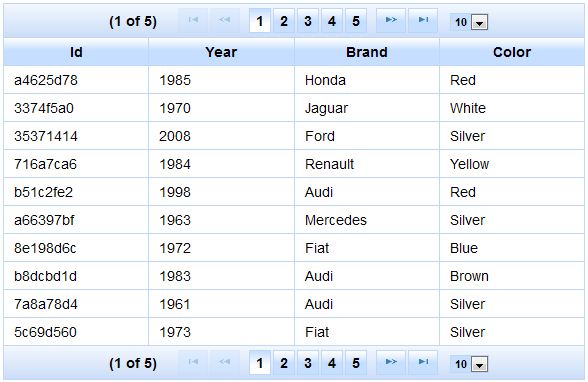
\includegraphics[width=0.75\textwidth]{/primefaces/datatable.png}
  \end{center}
  \fonte{PrimeFaces. Disponível em \url{https://www.primefaces.org/showcase/}}
\end{figure}

% ---
\subsection{Java Persistence API}\label{sec:jpa}
% ---

A API de Persistência do Java (JPA) possibilita o gerenciamento de dados relacionais nas aplicações Java através de um mapeamento objeto-relacional. Esse mapeamento é feito através de \emph{entidades}, \emph{i.e.}, objetos do domínio de persistência. Uma entidade representa uma tabela de um banco de dados no modelo relacional, e suas instâncias representam as linhas desta tabela. 

Segundo \citeonline{javaee7}, para ser considerada uma entidade, uma classe Java precisa:

\begin{enumerate}
  \item Possuir a anotação \texttt{javax.persistence.entity};
  \item Possuir ao menos um construtor sem argumentos com visibilidade \emph{public} ou \emph{protected};
  \item A classe, suas instâncias persistíveis e seus métodos não podem ser declarados \emph{final};
  \item Instâncias persistíveis devem ser declaradas como \emph{private}, \emph{protected} ou \emph{package private} e podem ser acessadas somente através dos métodos da classe.
\end{enumerate}

Tais restrições podem ser vistos na entidade \texttt{Empregado}, destacadas em forma de comentários no Algoritmo~\ref{alg:entity_emp}.

\begin{lstlisting}[caption={Entidade Empregado e seus mapeamentos.}, label={alg:entity_emp}]
@Entity // 1)
public class Empregado {
    @Id
    @Column(name="EMP_ID")
    private long id;
    private String nome;
    @ManyToOne
    private Setor setor; // 3 e 4
    
    public Empregado() {}  // 2
    // ...
}
\end{lstlisting}
%
Ainda com relação ao Algoritmo~\ref{alg:entity_emp}, é interessante observar as seguintes anotações:

\begin{itemize}
  \item \texttt{@Id} - indica que o campo é a chave primária da tabela.
  \item \texttt{@Column} - indica que o campo é uma coluna da tabela. Quando o parâmetro \texttt{name} não é especificado, assume-se que o nome da coluna é idêntico ao nome do campo (é o caso do campo \texttt{nome}).
  \item \texttt{@ManyToOne} - indica a relação entre as entidades \texttt{Empregado} e \texttt{Setor}. Neste caso, diversos empregados estão relacionados ao mesmo setor. \citeonline{keith2013} definem outras anotações utilizadas no relacionamento de entidades além de \texttt{@ManyToOne}. Para maiores detalhes, vide Anexo~\ref{anexo:jpa}.
\end{itemize}



% ---
%\subsection{Hibernate}
% ---

% ---
%\subsection{Spring}
% ---



\chapter{Análise e Projeto - Módulo de Inscrição}
% ----------------------------------------------------------

\citeonline{sommerville2011} explica que um \emph{processo de software} é um conjunto de atividades relacionadas que levam à produção de um produto de software. Embora existam diversos processos de software, todos devem incluir as seguintes atividades fundamentais: especificação, projeto e implementação, validação, e evolução do software. Cada uma destas atividades é uma tarefa complexa em si mesma e inclui subatividades.

Por não existir um modelo de processo de software único a ser utilizado na SeTIC, o autor decidiu-se por seguir algumas das melhores práticas estabelecidas pelo \emph{Rational Unified Process} (RUP), as quais já foram utilizadas em projetos anteriores em que o autor participou na SeTIC como estagiário (vide Anexo~\ref{anexo:rup}).

%: as atividades fundamentais supracitadas são executadas de forma iterativa, seguindo as boas práticas especificadas pelo \emph{Rational Unified Process} (RUP), um modelo de processo moderno e híbrido, derivado de trabalhos sobre a UML (Unified Modelling Language).

Ressalta-se que o desenvolvimento teve como inspiração o sistema existente. Fez-se uso de diversas tabelas já existentes, bem como dos campos presentes no formulário de inscrição. Não obstante, novas tabelas e campos foram criados, e a implementação das regras de negócio foi realizada pelo autor deste trabalho.


% ---
\section{Elicitação, Análise e Definição de Requisitos}
% ---

O desenvolvimento de um software/sistema segundo o modelo adotado pode ser dividido em diversos estágios. O primeiro consiste na elicitação, análise e definição de requisitos. Segundo \citeonline{sommerville2011}, os requisitos de um sistema são as descrições do que o sistema deve fazer, os serviços que oferece e as restrições a seu funcionamento. Esses requisitos refletem as necessidades dos clientes para um sistema que serve a uma finalidade determinada, como controlar um dispositivo, fazer um pedido ou encontrar informações. Esta etapa é muito importante pois, além de servir de base para as demais etapas, fornece um rumo a ser seguido e um objetivo a ser alcançado. Não menos importante, evita a implementação de funcionalidades desnecessárias.

A elicitação ou descoberta dos requisitos do sistema pode ser feita de diversas maneiras: entrevistas, cenários, casos de uso, etnografia, etc. A abordagem adotada aqui, comum aos demais sistemas desenvolvidos na SeTIC, foi a de realização de entrevistas abertas, isto é, uma série de questões relacionadas ao uso do sistema foi explorada junto ao cliente. Dessa forma, pôde-se obter uma melhor compreensão de suas necessidades.

Um conjunto de \emph{wireframes}, ou protótipos, das páginas do sistema foi desenvolvido\footnote{Utilizou-se um \emph{plugin} do WireframeSketcher feito para o Eclipse.} e apresentado com o objetivo de validar a estrutura, o conteúdo, as diversas funções e os diversos caminhos de interações dos usuários com o sistema. A confecção deste conjunto de \emph{wireframes} teve como base o sistema informatizado atualmente em uso. Em cima deste foram aplicadas todas as mudanças que se faziam necessárias e que justificam o desenvolvimento do novo sistema. A Figura~\ref{fig:wireframe} fornece um exemplo retirado deste conjunto: após o início da sessão no sistema, a página inicial exibida para o usuário Fulano apresenta um histórico de inscrições já realizadas por este usuário. Evidencia-se o uso de balões explicativos para agilizar o entendimento dos diversos elementos da página. Ressalta-se que o visual da página não é o foco do \emph{wireframe}, e sim o que ela permite que o usuário realize.

\begin{figure}[!ht]
  \caption{\label{fig:wireframe} \emph{Wireframe} que representa a página de inscrições realizadas pelo usuário Fulano após este ter feito \emph{login} no sistema. }
  \begin{center}
    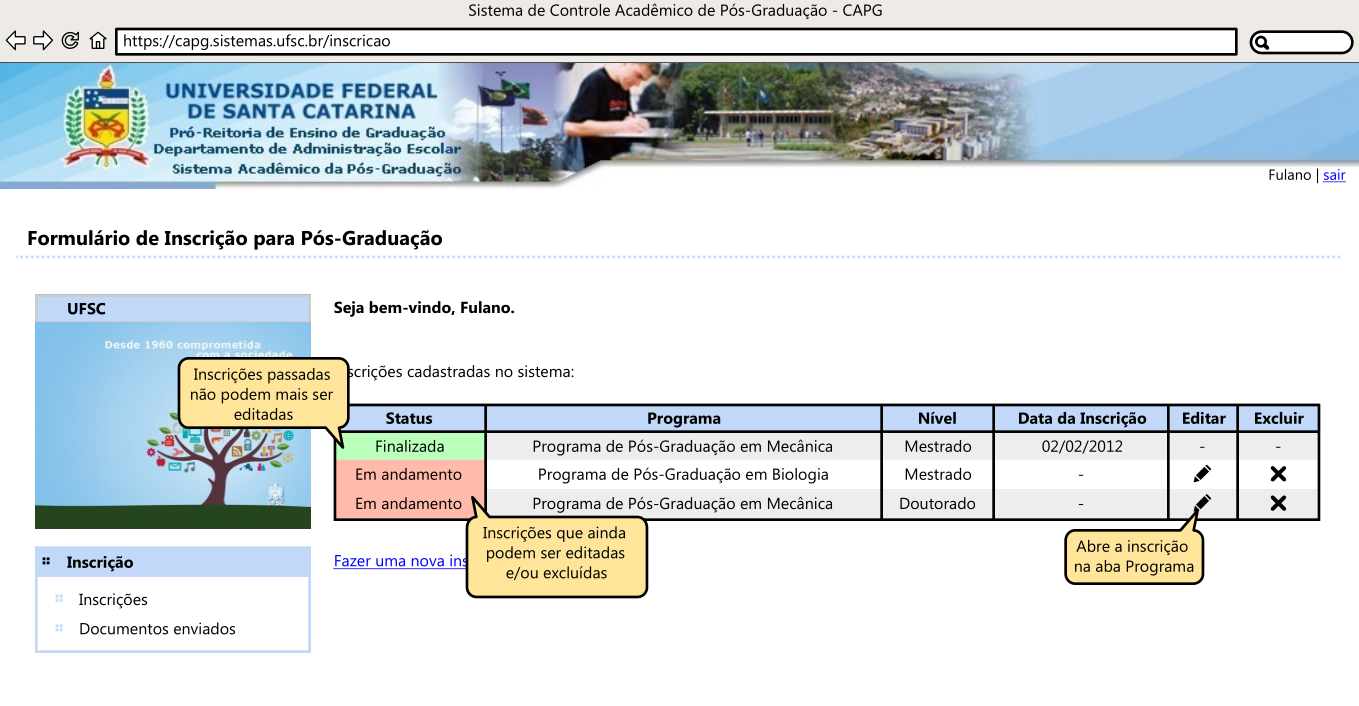
\includegraphics[width=1.0\textwidth]{/wireframe.png}
  \end{center}
  \fonte{Produzido pelo autor.}
\end{figure}

Na reunião com o cliente, os requisitos propostos e exemplificados nos \emph{wireframes} foram analisados. Destes, alguns foram removidos, outros adicionados. No fim, um conjunto de requisitos iniciais
%\footnote{Em princípio, segundo o modelo em cascata, cada estágio só se inicia após o término do anterior. Na prática, há uma sobreposição dos estágios: problemas com os requisitos são identificados durante o projeto e erros de programa aparecem durante a fase de operação e manutenção, exigindo uma reavaliação dos requisitos.}
 foi aprovado e serviu como uma especificação formal para o desenvolvimento do sistema. Embora a distinção entre os diferentes tipos de requisitos não seja tão clara, os requisitos de software são frequentemente classificados como \emph{funcionais} e \emph{não funcionais}. Essa classificação é abordada nos itens a seguir.

\subsection{Requisitos Funcionais}\label{sec:requisitos_funcionais}

Os requisitos funcionais descrevem os serviços que o sistema deve fornecer, como deve reagir a entradas específicas e como deve se comportar em determinadas situações. Visando o entendimento por todas as partes interessadas (\emph{stakeholders}), a especificação dos requisitos é feita aqui de forma abstrata (em alto nível).

\begin{description}
\item[Requisito 1 - Visualizar programas oferecidos.] O usuário poderá visualizar a lista de programas de pós-graduação oferecidos pela UFSC sem a necessidade de realizar \emph{login} no sistema.
\item[Requisito 2 - Realizar cadastro no CAS.] O usuário poderá se cadastrar no Sistema de Autenticação Centralizada a partir da página inicial do sistema.
\item[Requisito 3 - Acessar o sistema.] O usuário poderá acessar o sistema através de \emph{login}.
\item[Requisito 4 - Sair do sistema.] O usuário poderá sair do sistema a qualquer momento fazendo \emph{logout}.
\item[Requisito 5 - Salvar a inscrição.] O usuário poderá salvar as informações inseridas no formulário para um acesso futuro. Após o primeiro salvamento, o usuário receberá um número de inscrição.
\item[Requisito 6 - Alterar informações.] O usuário poderá alterar as informações inseridas durante todo o período de inscrição do programa selecionado, desde que não tenha finalizado a sua inscrição.
\item[Requisito 7 - Finalizar a inscrição.] O usuário poderá finalizar a sua inscrição. Após finalizada, os dados inseridos não poderão mais ser modificados.
\item[Requisito 8 - Receber um comprovante de inscrição.] Após finalizada a inscrição, o usuário receberá um comprovante de inscrição através do e-mail cadastrado.
\item[Requisito 9 - Importar dados do CAS.] Os dados que foram utilizados para fazer o cadastro no CAS deverão ser importados automaticamente.
\item[Requisito 10 - Importar dados de inscrições anteriores.] Ao iniciar uma nova inscrição, o usuário poderá importar dados pessoais e dados de contato da última inscrição realizada.
\item[Requisito 11 - Fazer \emph{upload} de arquivos.] O usuário poderá fazer o \emph{upload} de arquivos solicitados pelo programa escolhido.
\item[Requisito 12 - Importar arquivos.] O usuário poderá buscar arquivos utilizados em inscrições anteriores.
\item[Requisito 13 - Inserir informações.] O usuário poderá inserir diversos tipos de informações, as quais são agrupadas em dados do programa, pessoais, econômicos, de contato e de formação. Embora esses dados não estejam descritos em pormenores neste relatório, estavam presentes nos protótipos apresentados à PROPG na reunião de definição dos requisitos.
\end{description}


\subsection{Requisitos Não Funcionais}

Segundo \citeonline{sommerville2011}, os requisitos não funcionais são aqueles que não estão diretamente relacionados com os serviços específicos oferecidos pelo sistema a seus usuários. Relacionam-se às propriedades emergentes do sistema e definem restrições sobre a sua implementação. Foram identificados os seguintes requisitos:

\begin{itemize}
%\item O sistema deve possibilitar o acesso dos usuários durante todos os dias do ano para que possam imprimir comprovantes de inscrição.
\item Usuários do sistema devem autenticar-se utilizando o Sistema de Autenticação Centralizada (CAS).
\item A aplicação Web deve ser feita utilizando a linguagem de programação Java e as tecnologias que são comumente utilizadas no desenvolvimento Web com Java e que estão disponíveis na SeTIC (vide Seção~\ref{sec:java2e}).
\item A aplicação Web deve utilizar a estrutura e seguir o visual dos demais sistemas desenvolvidos na SeTIC\footnote{Este requisito se refere à versão \emph{desktop} da aplicação.}. Para tanto, deve-se utilizar o projeto denominado \emph{Projeto Base}, criado por desenvolvedores da SeTIC para o desenvolvimento de novos sistemas.
\item O sistema deve possuir uma interface responsiva, \emph{i.e.}, capaz de ajustar a disposição do conteúdo em função das dimensões da janela do navegador e do tipo de dispositivo utilizado (\emph{desktop} ou móvel). 
\end{itemize}

% ---
\section{Projeto do Sistema}
% ---

O segundo estágio do modelo de desenvolvimento de software adotado consiste em desenvolver a arquitetura geral do sistema. Aqui descrevem-se as principais abstrações do sistema e seus relacionamentos através dos diagramas de casos de uso e de classes.

\subsection{Diagrama de Casos de Uso}\label{sec:casos_uso}

Diagramas de casos de uso fornecem uma representação em alto nível da interação entre os diversos usuários (chamados de atores) com o sistema. A Figura~\ref{fig:use_cases} abaixo relaciona os casos de uso identificados para o sistema de inscrição. As interações são representadas por elipses e os atores por bonecos palito. Identificam-se os seguintes atores:

\begin{itemize}
  \item \textbf{Candidato}, o principal ator e que atua em todos os casos de uso identificados.
  \item \textbf{CAS}, ator que interage apenas com os casos de uso relacionados à autenticação do ator Candidato.
  \item \textbf{Sybase}, uma interface para o sistema de gerenciamento do banco de dados e que atua em todos os casos de uso que necessitam de acesso ao banco de dados.
  \item \textbf{Storage}, uma interface para o repositório de documentos enviados pelo ator Candidato.
\end{itemize}

Nota-se também que o caso de uso \emph{verificar inscrição} é o único caso de uso que interage com apenas um ator. Isto se deve ao fato de que a verificação de campos não-preenchidos e de campos com erros de preenchimento é feita em parte pelo JSF e em parte no \emph{bean} associado a \emph{view} de inscrição (ambos na camada Web).

\begin{figure}[!ht]
  \caption{\label{fig:use_cases} Casos de uso identificados no sistema.}
  \begin{center}
    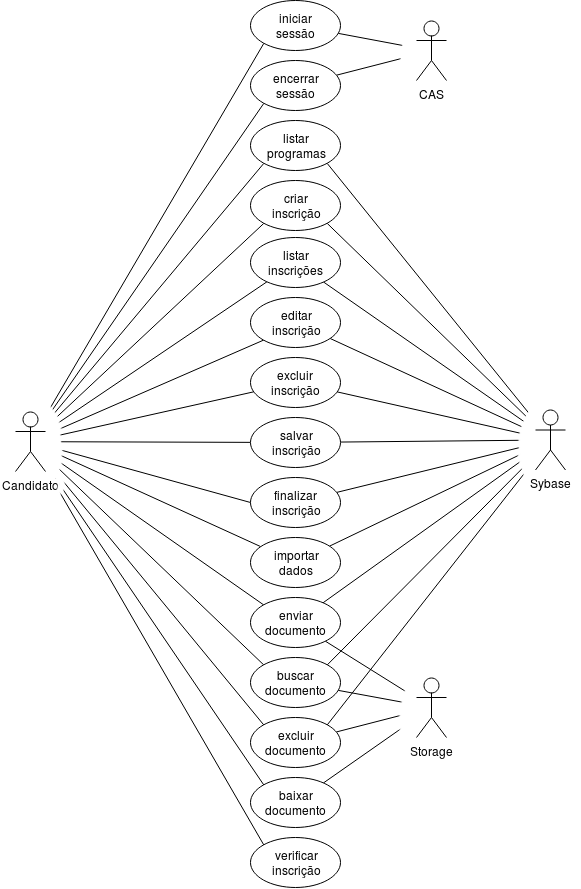
\includegraphics[width=0.9\textwidth]{/uml/use_cases.png}
  \end{center}
  \fonte{Elaborada pelo autor.}%
\end{figure}

% ---
\subsection{Diagrama de Visão Geral de Interação}
% ---

Introduzido na versão 2.0 da UML, este diagrama é uma versão modificada do diagrama de atividades, no qual ao invés de ações ou atividades, os nós correspondem a \emph{interações} que são modeladas em outros diagramas. Sua finalidade é modelar as sequências possíveis de ocorrência das interações identificadas. Uma possível aplicação do diagrama de visão geral de interação é a modelagem do fluxo entre as interações associadas aos casos de uso identificados anteriormente. 

O fluxo de execução pode ser visto na Figura~\ref{fig:interaction}. Identificam-se os seguintes elementos:

\begin{itemize}
  \item \textbf{Nós de uso de interação}, que referenciam as interações associadas aos casos de uso.
  \item \textbf{Nós de decisão}, responsáveis por receber o fluxo a partir de uma ou mais arestas e selecionar a direção do fluxo de execução de acordo com as guardas.
  \item \textbf{Guardas}, ou condições booleanas escritas entre colchetes, condicionam a saída do nó de decisão.
  \item \textbf{Nó inicial}, representado por um círculo preto, a partir do qual inicia-se o fluxo de execução.
  \item \textbf{Nó final}, representado por um círculo preto inscrito em uma circunferência preta, no qual termina o fluxo de execução. 
\end{itemize}

\begin{figure}[!ht]
  \caption{\label{fig:interaction} Interação entre os ``casos de uso'' do sistema. Algumas guardas foram omitidas para não saturar o diagrama.}
  \begin{center}
    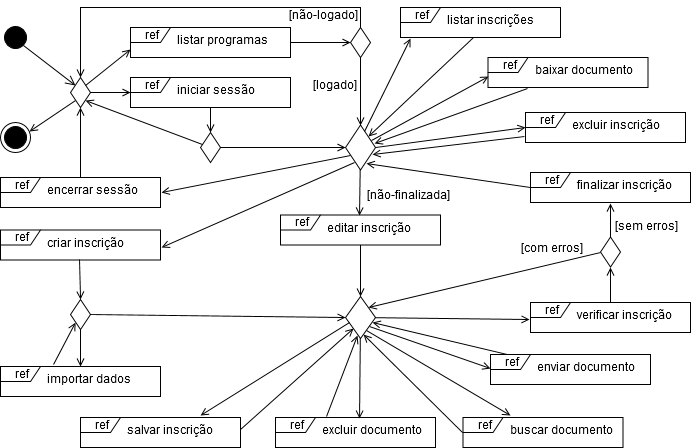
\includegraphics[width=1.0\textwidth]{/uml/interaction.png}
  \end{center}
  \fonte{Elaborada pelo autor.}%
\end{figure}

% ---
\subsection{Diagrama de Classes}
% ---

Um diagrama de classes é responsável por mostrar as diversas classes de uma aplicação e as associações (agregação, composição, generalização e dependências) entre elas.

O diagrama de classes do sistema foi dividido em duas imagens por questão de espaço. A Figura~\ref{fig:uml_er1} mostra as classes envolvidas na obtenção dos programas disponíveis em uma determinada data. Pode-se perceber uma associação de generalização entre as classes \texttt{ProgramasService} e \texttt{ProgramasServiceImpl} e dependências entre as classes \texttt{ProgramasBean} e \texttt{ProgramaAux}, e \texttt{ProgramasBean} e \texttt{ProgramasService}.

\begin{figure}[!ht]
  \caption{\label{fig:uml_er1} Modelo entidade-relacionamento relacionado à obtenção de programas. }
  \begin{center}
    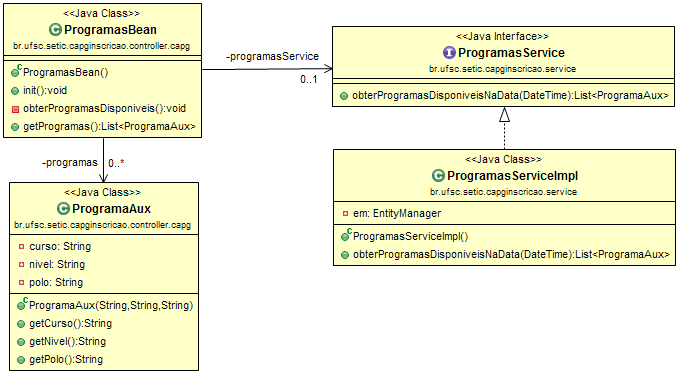
\includegraphics[width=1.0\textwidth]{/uml/programas.png}
  \end{center}
  \fonte{Elaborada pelo autor com a ferramenta ObjectAid UML Explorer.}%
\end{figure}

A Figura~\ref{fig:uml_er2} ilustra a classe \texttt{InscricoesBean} e algumas das suas associações de dependência. As classes \texttt{Curso} e \texttt{Nivel} são entidades e estão relacionadas entre si. \texttt{InscricoesService} é uma interface que provê serviços à classe \texttt{InscricoesBean}. Finalmente, \texttt{InscricaoAux} é uma classe auxiliar que é utilizada junto à \emph{view} para exibir informações das inscrições cadastradas para um determinado usuário.

\begin{landscape}
\begin{figure}[!ht]
  \caption{\label{fig:uml_er2} Modelo entidade-relacionamento relacionado às inscrições. }
  \begin{center}
    \includegraphics[scale=0.40]{/uml/inscricoes.png}
  \end{center}
  \fonte{Elaborada pelo autor com a ferramenta ObjectAid UML Explorer.}%
\end{figure}
\end{landscape}

% ---
\subsection{Diagrama de Entidade-Relacionamento}
% ---

Tendo em vista o requisito funcional de permitir ao candidato enviar e importar documentos, foi desenvolvido o modelo de relacionamento entre entidades exibido na Figura~\ref{fig:uml_storage}.

\colorbox{yellow}{\textbf{TODO:}} substituir os nomes das tabelas e campos no modelo entidade-relacionamento abaixo por nomes mais genéricos próprios de um projeto.

\begin{figure}[!ht]
  \caption{\label{fig:uml_storage} Modelo entidade-relacionamento associado ao salvamento de documentos. }
  \begin{center}
    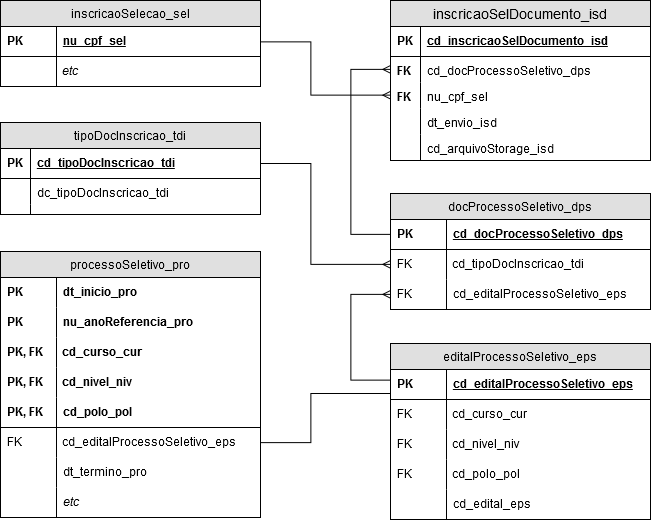
\includegraphics[width=1.0\textwidth]{/uml/storage.png}
  \end{center}
  \fonte{Elaborada pelo autor.}%
\end{figure}


Em relação às entidades mostradas na Figura~\ref{fig:uml_storage}, as tabelas \texttt{inscricaoSelecao\_sel}, \texttt{processoSeletivo\_pro} e \texttt{editalProcessoSeletivo\_eps} já existiam na base de dados. A primeira engloba os dados pessoais do candidato; as outras duas representam processos seletivos e seus respectivos editais. As demais entidades foram modeladas para atender aos requisitos 11 e 12 (vide Seção~\ref{sec:requisitos_funcionais}):

\begin{itemize}
  \item \texttt{tipoDocInscricao\_tdi} - contém os tipos dos documentos obrigatórios para a inscrição nos diversos programas, \emph{e.g.}, histórico escolar, diploma de graduação, RG, \emph{etc}.
  \item \texttt{inscricaoSelDocumento\_isd} - entidade que armazena o código dos documentos enviados por cada candidato. Os documentos propriamente ditos são armazenados em um repositório e seus identificadores salvos no campo \texttt{cd\_arquivoStorage\_isd}. Pode-se obter, por exemplo, uma lista de códigos de documentos enviados por um determinado candidato e, a partir da relação com a entidade \texttt{docProcessoSeletivo\_dps}, qual o tipo de cada documento e a qual processo seletivo pertence.
  \item \texttt{docProcessoSeletivo\_dps} - entidade associativa entre as entidades \texttt{tipoDocInscricao\_tdi} e \texttt{editalProcessoSeletivo\_eps}, com chave própria.
\end{itemize}

% ---
\chapter{Implementação}
% ----------------------------------------------------------

% ---
\section{Configuração do projeto}\label{sec:config}
% ---

Após definida a estrutura inicial do sistema, deu-se início ao processo de implementação. O projeto foi configurado para atender às necessidades do sistema. Além de arquivos de configuração, diversos pacotes foram criados para a separação lógica das classes, como pode ser visto na Figura~\ref{fig:src_explorer}.

\begin{figure}[!ht]
  \caption{\label{fig:src_explorer} Alguns pacotes e classes da aplicação vistos no Eclipse. }
  \begin{center}
    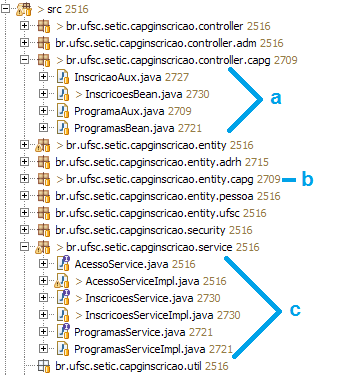
\includegraphics[width=0.6\textwidth]{/src_explorer.png}
  \end{center}
  \fonte{Elaborada pelo autor.}
\end{figure}

O pacote \texttt{(a)} é composto de \emph{beans} e classes auxiliares da camada Web (vide Seção~\ref{sec:camada-web}) que, em conjunto com os arquivos .xhtml, são responsáveis por gerar as páginas da aplicação.

O mapeamento objeto-relacional se encontra no pacote destacado por \texttt{(b)}. Aqui se encontram as classes das inúmeras entidades do sistema (vide Seção~\ref{sec:camada-negocio}) e, por serem muitas, não foram incluídas na imagem.

As classes representadas por \texttt{(c)}, assim como as classes do item \texttt{(b)}, pertencem à camada de negócios. São classes ditas de serviço, responsáveis pelas operações básicas de persistência: \emph{Create}, \emph{Read}, \emph{Update}, \emph{Delete}, comumente abreaviadas por CRUD. Na Figura~\ref{fig:src_explorer}, as classes \texttt{AcessoService}, \texttt{InscricoesService} e \texttt{ProgramasService} são interfaces\footnote{Em Java, uma interface é um tipo abstrato que especifica um comportamento que deve ser implementado.}, enquanto que \texttt{AcessoServiceImpl}, \texttt{InscricoesServiceImpl} e \texttt{ProgramasServiceImpl} representam suas implementações.



Para ilustrar a operação \emph{read}, o Algoritmo~\ref{alg:programas_disponiveis} contém o método que obtém a lista de programas disponíveis em uma determinada data. Percebe-se que o tipo do elemento contido na lista é um \texttt{ProgramaAux}, uma das classes auxialiares mencionadas no item \texttt{(a)}. A instância do \texttt{EntityManager}, que está associada a um contexto de persistência, é representada por \texttt{em}.
%TODO - referenciar JPA


%\begin{landscape}
\begin{lstlisting}[language=java, caption={Obtenção da lista de programas disponíveis.}, label={alg:programas_disponiveis}]
public List<ProgramaAux>
obterProgramasDisponiveisNaData(DateTime data) {
    StringBuffer query = new StringBuffer();
    query.append("SELECT new br.ufsc...ProgramaAux(");
    query.append("ps.curso.nome, ps.nivel.descricao, ");
    query.append("ps.polo.nome) ");
    query.append("FROM ProcessoSeletivo ps ");
    query.append("WHERE :dt BETWEEN ps.dtInicioProcesso ");
    query.append("AND ps.dtTerminoProcesso ");
    query.append("ORDER BY ps.curso");

    return em.createQuery(query.toString(),
                          ProgramaAux.class)
            .setParameter("dt", data.toLocalDateTime())
            .getResultList();
}
\end{lstlisting}
\fonte{Produzido pelo autor.}%
%\end{landscape}


Ressalta-se que a maioria das classes presentes na Figura~\ref{fig:src_explorer} já existiam no Projeto Base e provêm funcionalidades como segurança (através do Spring), acesso a Web Services, comunição com a base de dados Centura, validadores e conversores do JSF, \emph{etc}.


% ---
\section{Dispositivos móveis}\label{sec:mobile}
% ---
Não é novidade que a utilização de dispositivos móveis para a navegação na internet tem crescido nos últimos anos. Segundo dados obtidos na própria SeTIC, aproximadamente 30\% dos usuários que fizeram inscrição nos sistemas NDI (Núcleo de Desenvolvimento Infantil) e CAPL (Colégio da Aplicação) em 2017 utilizaram dispositivos móveis (celulares e tablets).

A adaptação da interface do sistema para a utilização em dispositivos móveis é um requisito não-funcional, cuja implementação teve de levar em consideração duas abordagens:

\begin{itemize}
  \item A utilização de um \emph{add-on} da biblioteca PrimeFaces chamado PrimeFaces Mobile (PFM), o qual permite a criação de aplicações Web baseadas em JSF otimizadas para o uso em dispositivos móveis. Nesta abordagem, utilizam-se \emph{views} separadas para navegadores de dispositivos móveis e para navegadores comuns, e reutilizam-se os métodos da camada de negócio da aplicação. Embora isso permita maior usabilidade e experiência mais agradável para usuários acostumados a utilizar aplicativos móveis, a duplicação de código dificulta a manutenibilidade da aplicação.
  \item A utilização de páginas responsivas: as mesmas \emph{views} são utilizadas em navegadores comuns e navegadores de dispositivos móveis, e a disposição dos elementos é controlada a partir de \emph{CSS media queries}.
\end{itemize}
%
Tendo em vista a manutenibilidade do código, optou-se pela segunda abordagem. As imagens utilizadas na exemplificação das funcionalidades mostradas a seguir foram obtidas em navegadores comuns. Imagens obtidas em um navegador de um dispositivo móvel\footnote{Motorola Moto G5 com resolução de 1920x1080 pixels.} podem ser vistas no Anexo~\ref{anexo:mobile}.


% ---
\section{Funcionalidades}\label{sec:funcionalidades}
% ---

A Tabela~\ref{tab:casos-uso} mostra um mapeamento entre os casos de uso identificados para o ator Candidato (vide Seção~\ref{sec:casos_uso}) e as páginas nas quais foram implementados. A implementação de cada item está descrita nas subseções a seguir.


\begin{table}[!htb]
  \IBGEtab{%
    \caption{Casos de uso implementados e respectivas páginas envolvidas.}%
    \label{tab:casos-uso}
  }{
    \begin{tabular}{ll}
      \toprule
      \textbf{Caso de Uso} & \textbf{Página da Aplicação} \\
      \midrule \midrule
      Listar programas     & \texttt{programas.xhtml} \\
      \midrule 
      Iniciar sessão       & \texttt{login.xhtml} \\
      \midrule
      Encerrar sessão      & A partir de qualquer página \\
      \midrule
      Listar inscrições    & \multirow{4}{*}{\texttt{inscricoes.xhtml}} \\
      Criar inscrição      & \\
      Editar inscrição     & \\
      Excluir inscrição    & \\
      \midrule
      Enviar documento     & \texttt{enviar\_documento.xhtml} \\
      \midrule
      Buscar documento     & \texttt{buscar\_documento.xhtml} \\
      \midrule
      Baixar documento     & \texttt{documentos\_enviados.hxtml} \\
      \midrule
      Excluir documento    & \multirow{5}{*}{\texttt{inscricao.xhtml}} \\
      Importar dados       & \\
      Salvar inscrição     & \\
      Finalizar inscrição  & \\
      Verificar inscrição  & \\
      \bottomrule
    \end{tabular} 
  }{
    \fonte{Elaborada pelo autor.}%
    %\nota{Utiliza a caixa de diálogo modal \boxcolor{\texttt{nome_da_caixa.html}}.}%
    %\nota[Anotações]{Uma anotação adicional, seguida de várias outras.}%
  }
\end{table}



% ---
\subsection{Lista de programas disponíveis}\label{sec:programas_disponiveis}
% ---
%Como pode ser visto na Tabela~\ref{tab:casos-uso}, a visualização dos programas disponíveis possui uma página própria, \texttt{programas.xhtml}.
O acesso à lista de programas disponíveis para a inscrição é feita a partir da página inicial da aplicação, conforme destacado na Figura~\ref{fig:acesso_programas} por um retângulo verde. O candidato não precisa estar logado no sistema para acessá-la. A lista exibe os programas, os níveis e os polos que estão com inscrições abertas no momento do acesso à página (vide Figura~\ref{fig:programas_disponiveis}).

\begin{figure}[!ht]
  \caption{\label{fig:acesso_programas} Acesso à lista de programas disponíveis em destaque. }
  \begin{center}
    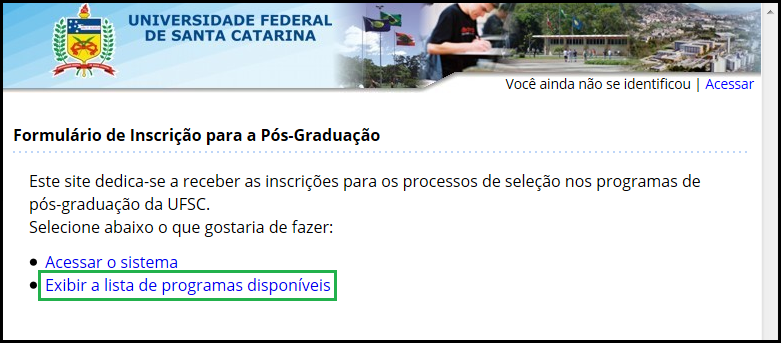
\includegraphics[width=1.0\textwidth]{/app/acesso_programas.png}
  \end{center}
  \fonte{Elaborada pelo autor.}
\end{figure}



\begin{figure}[!ht]
  \caption{\label{fig:programas_disponiveis} Lista de programas disponíveis para inscrição. }
  \begin{center}
    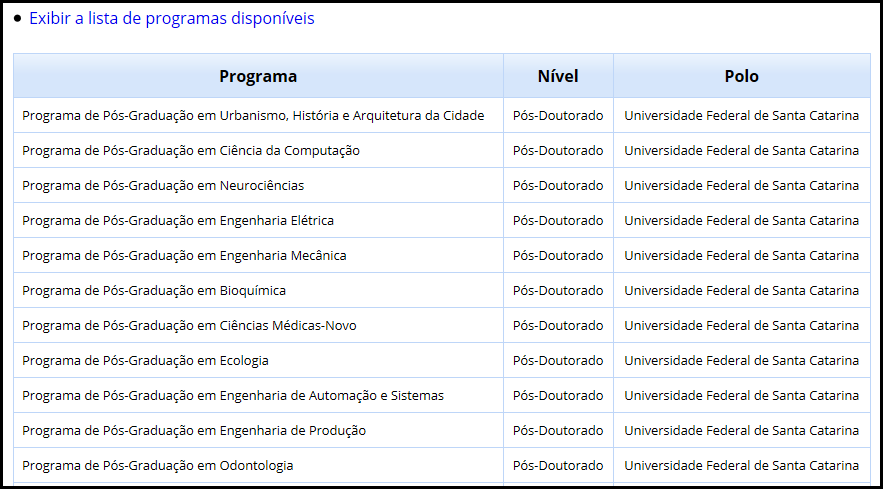
\includegraphics[width=1.0\textwidth]{/app/programas_disponiveis.png}
  \end{center}
  \fonte{Elaborada pelo autor.}
\end{figure}




% ---
\subsection{Autenticação no sistema}\label{sec:autenticacao}
% ---
Como pode ser visto no diagrama de casos de uso, Figura~\ref{fig:use_cases}, o cadastro e a autenticação no sistema são feitos através do Sistema de Autenticação Centralizada (CAS), que permite a navegação entre os diversos sistemas da UFSC com apenas uma autenticação. Ao clicar nos links de acesso (vide destaque na Figura~\ref{fig:acesso_sistema}), o candidato é automaticamente transferido à página do CAS (vide Figura~\ref{fig:autenticacao}), onde pode cadastrar-se e autenticar-se perante o sistema. Salienta-se que o CAS é um sistema já existente e utilizado por diversos outros sistemas da UFSC, e que o CAPG Inscrição atua apenas como cliente.


\begin{figure}[!ht]
  \caption{\label{fig:acesso_sistema} Acesso ao sistema de inscrição do CAPG. }
  \begin{center}
    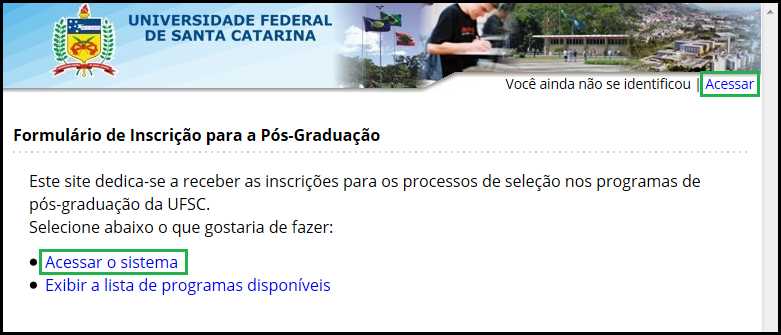
\includegraphics[width=1.0\textwidth]{/app/acesso_sistema.png}
  \end{center}
  \fonte{Elaborada pelo autor.}
\end{figure}

Após autenticado, o candidato é automaticamente transferido para a página de inscrições (vide Figura~\ref{fig:inscricoes}). Nesta, destaca-se o nome do usuário autenticado no sistema por um retângulo verde, e à sua direita o link para encerrar a sua sessão no sistema.

\begin{figure}[!ht]
  \caption{\label{fig:autenticacao} Cadastro e autenticação no CAS. }
  \begin{center}
    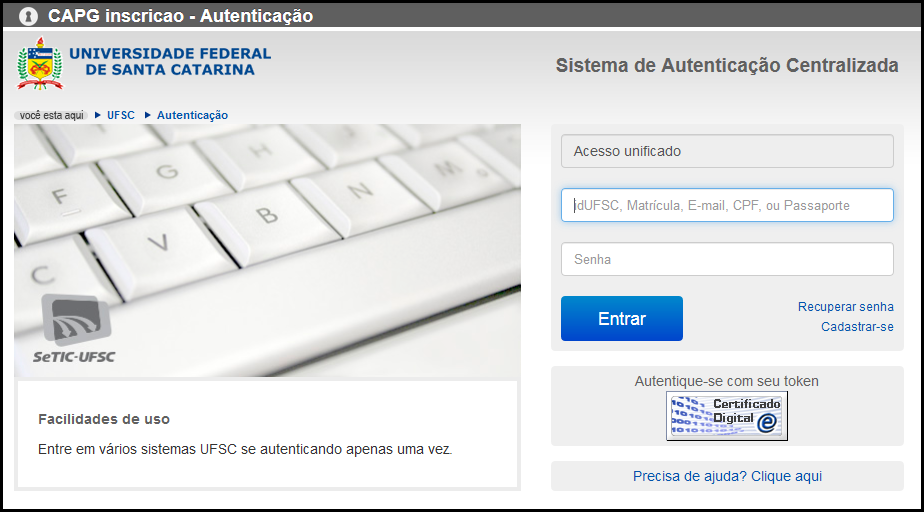
\includegraphics[width=1.0\textwidth]{/app/autenticacao.png}
  \end{center}
  \fonte{Elaborada pelo autor.}
\end{figure}


\begin{figure}[!ht]
  \caption{\label{fig:inscricoes} Lista de inscrições do candidato. Em destaque: encerramento da sessão.}
  \begin{center}
    \includegraphics[width=1.0\textwidth]{/app/inscricoes.png}
  \end{center}
  \fonte{Elaborada pelo autor.}
\end{figure}

% ---
\subsection{Gerenciamento de inscrições}\label{sec:gerenciamento_inscricoes}
% ---

O usuário autenticado no sistema tem acesso ao histórico de inscrições realizadas. Neste histórico, identificam-se o programa, o nível e a data de finalização da inscrição, como pode ser visto na tabela da Figura~\ref{fig:inscricoes}. Cada inscrição possui ainda um \emph{status}: 

\begin{itemize}
  \item \textbf{Finalizada} -- inscrição pertencente a um processo seletivo passado que não pode ser editada ou excluída.
  \item \textbf{Em andamento} -- inscrição pertencente a um processo seletivo em vigência que pode ser editada e/ou excluída.
\end{itemize}

Ressalta-se que a tabela com o histórico de inscrições não é visível para candidatos que nunca realizaram uma inscrição em algum dos processos seletivos para cursos de pós-graduação da UFSC. Para estes, apenas o link \texttt{Fazer uma nova inscrição}\footnote{Link na parte inferior da tabela da Figura~\ref{fig:inscricoes}.} estará disponível.


% ---
\subsection{Criação de uma inscrição}\label{sec:criacao_inscricao}
% ---

É possível criar uma nova inscrição a partir da tela de inscrições. Ao fazê-lo, o candidato se depara com uma tela tal qual a da Figura~\ref{fig:criar_inscricao}, na qual identificam-se alguns pontos:

\begin{itemize}
  \item No \emph{cabeçalho} da página encontram-se algumas mensagens informativas que têm o propósito de auxiliar o usuário sobre a utilização da aplicação.
  \item No \emph{corpo} da página encontra-se um componente da biblioteca PrimeFaces chamado \texttt{AccordionPanel}\footnote{Vide \href{https://www.primefaces.org/showcase/ui/panel/accordionPanel.xhtml}{https://www.primefaces.org/showcase/ui/panel/accordionPanel.xhtml}.}, composto de diversas abas. Quando uma aba recebe um clique do mouse, o seu conteúdo é exibido progressivamente (daí a referência a um acordeão).
  \item No \emph{rodapé} da página encontram-se os botões de ação \texttt{Salvar}, \texttt{Validar} e \texttt{Finalizar}. O botão \texttt{Salvar} é habilitado após o preenchimento do campo \texttt{Polo}, e salva as informações fornecidas pelo usuário na base de dados. Deve-se atentar para o fato de que as informações fornecidas pelos usuários não são salvas automaticamente, daí o uso do botão. A utilização dos demais botões será explicada na seção \ref{sec:validacao}.
\end{itemize}


\begin{figure}[!ht]
  \caption{\label{fig:criar_inscricao} Criação de uma nova inscrição.}
  \begin{center}
    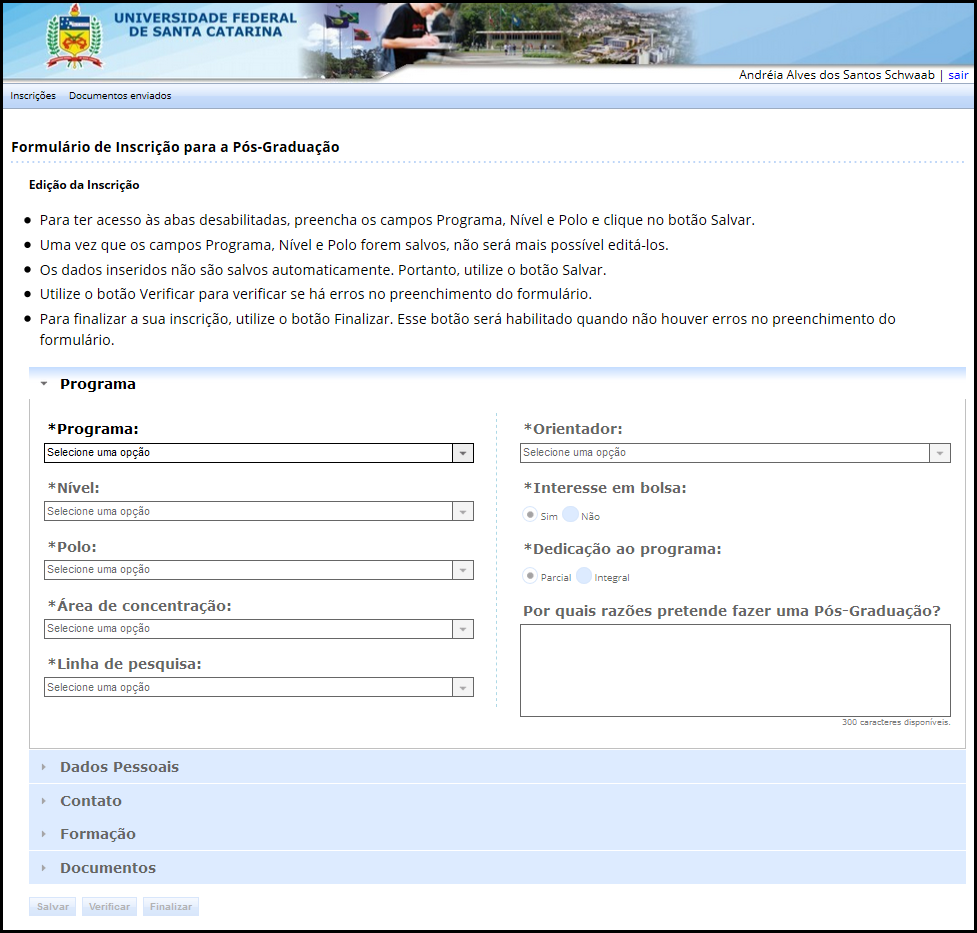
\includegraphics[width=1.0\textwidth]{/app/criar_inscricao.png}
  \end{center}
  \fonte{Elaborada pelo autor.}
\end{figure}

Nota-se que, com exceção da aba \texttt{Programa}, as demais estão desabilitadas no início do preenchimento de uma inscrição. Para habilitá-las, é preciso preencher os campos \texttt{Programa}, \texttt{Nível} e \texttt{Polo}, e clicar no botão \texttt{Salvar}. Após o salvamento, o candidato terá a opção de importar os dados da última inscrição por si realizada, caso exista (vide Figura~\ref{fig:importar_dados}). A partir deste ponto, os casos de uso \emph{criar inscrição} e \emph{editar inscrição} têm as mesmas funcionalidades.


\begin{figure}[!ht]
  \caption{\label{fig:importar_dados} Importação de dados na criação de uma nova inscrição.}
  \begin{center}
    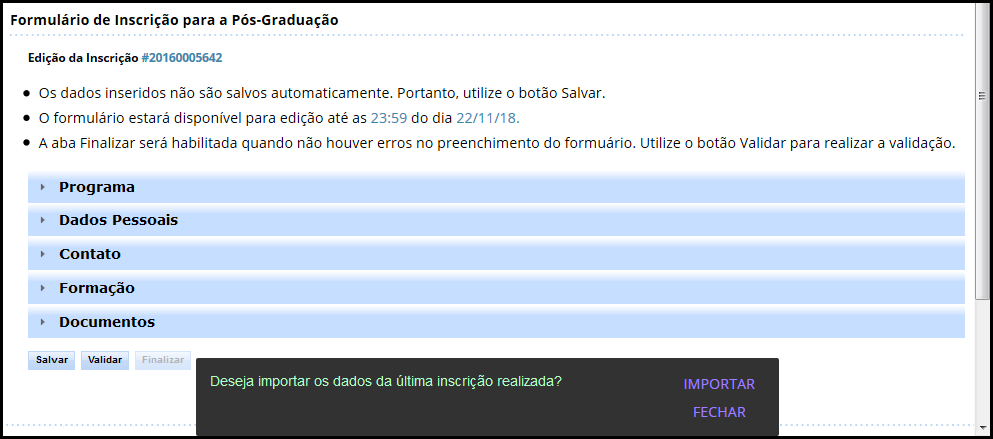
\includegraphics[width=1.0\textwidth]{/app/importar_dados.png}
  \end{center}
  \fonte{Elaborada pelo autor.}
\end{figure}


% ---
\subsection{Edição de uma inscrição}\label{sec:edicao_inscricao}
% ---

A Figura~\ref{fig:importar_dados} ilustra uma página típica de quando se inicia a edição de uma inscrição, com exceção da mensagem de importação de dados. Nota-se que, ao contrário da página inicial da criação de uma nova inscrição, o número da inscrição e a data limítrofe para a finalização da inscrição são exibidas no cabeçalho da página.

A Figura~\ref{fig:dados_pessoais_desktop} exibe os campos da aba \texttt{Dados Pessoais} preenchidos com dados fictícios. É importante ressaltar que alguns dos campos dependem do preenchimento do campo \texttt{País de origem}:
\begin{itemize}
  \item Quando o país de origem selecionado for \texttt{Brasil}, os campos \texttt{Naturalidade} e \texttt{Município de trabalho} são capazes de completar automaticamente o valor inserido pelo usuário\footnote{Utiliza-se um componente PrimeFaces chamado \texttt{AutoComplete}.}. Para isso, requerem que o usuário insira ao menos três caracteres.
  \item Ao escolher um país estrangeiro, os campos \texttt{Naturalidade} e \texttt{Município de trabalho} tornam-se campos de entrada de texto normais, sem a funcionalidade de auto-completar a entrada fornecida. Ainda, os campos \texttt{Número do RG}, \texttt{UF} e \texttt{Órgão expedidor} são substituídos pelos campos \texttt{Número do passaporte} e \texttt{Validade do passaporte}, e o campo \texttt{CPF} deixa de ser obrigatório.
\end{itemize}
%
\begin{figure}[!ht]
  \caption{\label{fig:dados_pessoais_desktop} Campos da aba \texttt{Dados Pessoais}.}
  \begin{center}
    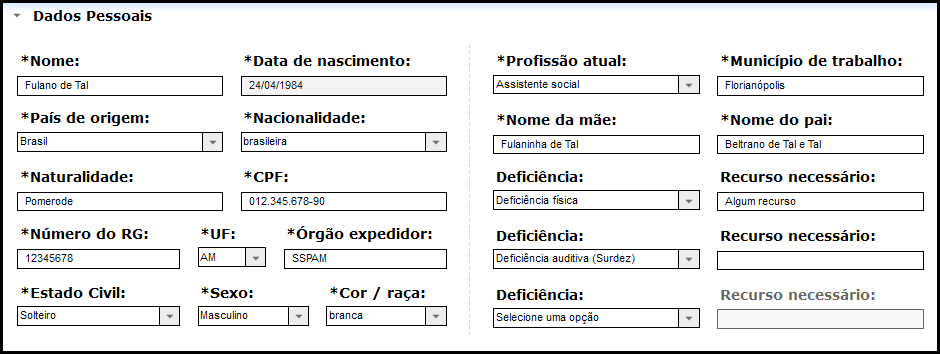
\includegraphics[width=1.0\textwidth]{/app/dados_pessoais_desktop.png}
  \end{center}
  \fonte{Elaborada pelo autor.}
\end{figure}
%
Os pares formados pelos campos \texttt{Deficiência} e \texttt{Recurso necessário} têm o seguinte funcionamento: 

\begin{itemize}
  \item Inicialmente, apenas o campo \texttt{Deficiência} do primeiro par está habilitado.
  \item Se o usuário selecionar um valor para um campo \texttt{Deficiência}, habilita-se o campo \texttt{Recurso necessário} do seu par e o campo \texttt{Deficiência} do par seguinte.
  \item Se o usuário limpar algum campo \texttt{Deficiência}, então o campo \texttt{Recurso necessário} do seu par e todos os pares seguintes serão desabilitados. 
  \item Podem existir ao todo três pares.
\end{itemize}

O preenchimento da aba \texttt{Contato} depende do campo \texttt{País}. A Figura~\ref{fig:contato_desktop} exibe duas situações: 
%
\begin{enumerate}[label=(\alph*)]
  \item Se o endereço for nacional, então os campos \texttt{Município}, \texttt{Bairro} e \texttt{Logradouro} serão automaticamente preenchidos quando o usuário preencher o campo \texttt{CEP} e pressionar a tecla \texttt{<TAB>} (ou clicar fora do campo).
  \item Se o endereço for internacional, então o campo \texttt{CEP} é desabilitado e o usuário deve preencher os campos \texttt{Município}, \texttt{Bairro} e \texttt{Logradouro}.
\end{enumerate}
%
\begin{figure}[!ht]
  \caption{\label{fig:contato_desktop} Preenchimento da aba \texttt{Contato}. Em \texttt{(a)}, tem-se um endereço nacional. Em \texttt{(b)}, internacional.}
  \begin{center}
    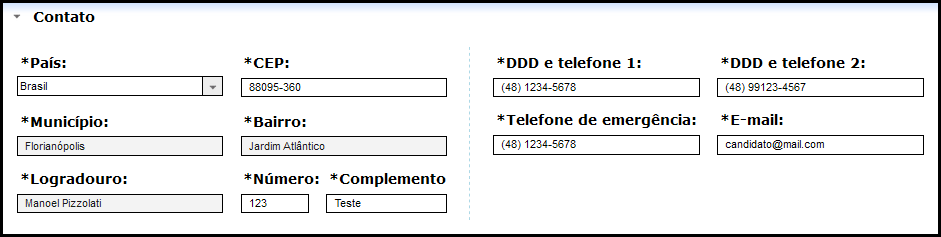
\includegraphics[width=1.0\textwidth]{/app/contato_desktop.png}
  \end{center}
  \fonte{Elaborada pelo autor.}
\end{figure}
%
Ainda, os campos relacionados a números de telefone são automaticamente formatados conforme o usuário insere os números.

Os candidatos podem adicionar cursos de formação já concluídos ou em andamento na aba \texttt{Formação}, através do link \texttt{Adicionar curso} (vide Figuras~\ref{fig:formacao_desktop}~e~\ref{fig:adicionar_curso}). Nesta última, se a caixa \texttt{Instituição nacional} estiver selecionada, então o campo \texttt{Instituição} completa automaticamente o valor inserido pelo usuário (a partir de três caracteres).

\begin{figure}[!ht]
  \caption{\label{fig:formacao_desktop} Campos da aba \texttt{Formação}.}
  \begin{center}
    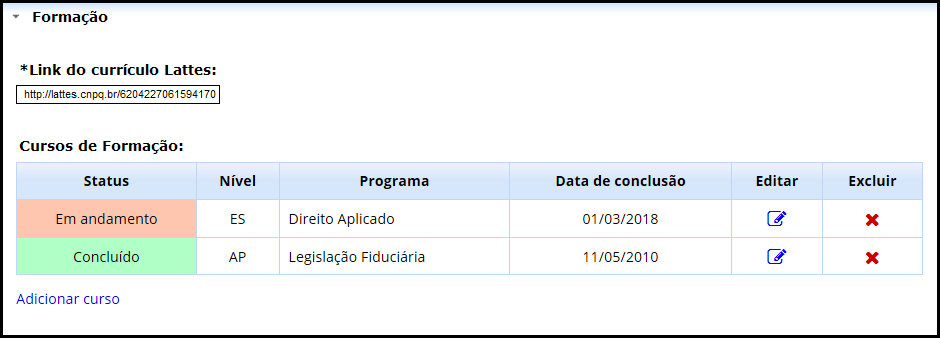
\includegraphics[width=1.0\textwidth]{/app/formacao_desktop.png}
  \end{center}
  \fonte{Elaborada pelo autor.}
\end{figure}


\begin{figure}[!ht]
  \caption{\label{fig:adicionar_curso} Caixa de diálogo modal que permite a adição de um curso de formação.}
  \begin{center}
    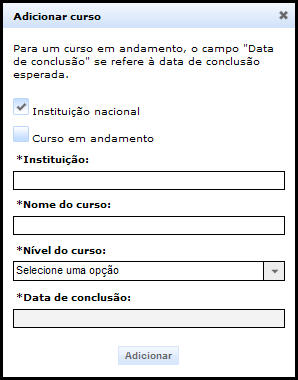
\includegraphics[width=0.4\textwidth]{/app/adicionar_curso.png}
  \end{center}
  \fonte{Elaborada pelo autor.}
\end{figure}



% ---
\subsection{Envio de documentos}\label{sec:envio_documentos}
% ---

Uma das principais funcionalidades providas por este sistema é permitir que o candidato faça o envio de documentos. Não somente se reduz a quantidade de papéis que ficariam armazenados nas secretarias dos cursos (economizando espaço), como também potencializa-se a segurança dos documentos (documentos em papel estão sempre sujeitos a danos e avarias) e facilita-se a sua busca. Essa funcionalidade está implementada na aba \texttt{Documentos}, como pode ser visto na Figura~\ref{fig:documentos_desktop}. As linhas da tabela representam os documentos que são exigidos pela secretaria a qual o programa escolhido está vinculado. No exemplo fictício mostrado, são exigidos três documentos, dois dos quais já foram enviados, e um está pendente.
%
\begin{figure}[!ht]
  \caption{\label{fig:documentos_desktop} Campos da aba \texttt{Documentos}.}
  \begin{center}
    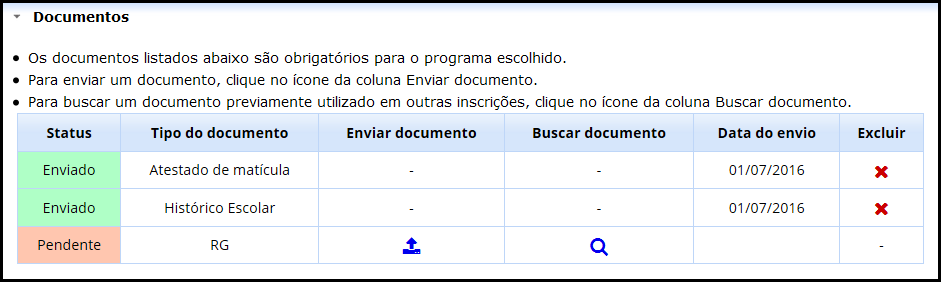
\includegraphics[width=1.0\textwidth]{/app/documentos_desktop.png}
  \end{center}
  \fonte{Elaborada pelo autor.}
\end{figure}

A partir da tabela, pode-se \emph{enviar} novos documentos (vide Figura~\ref{fig:enviar_documento_desktop}) e \emph{buscar} documentos de inscrições passadas realizadas pelo candidato (vide Figura~\ref{fig:buscar_documento_desktop}).
%
\begin{figure}[!ht]
  \caption{\label{fig:enviar_documento_desktop} Envio de documentos.}
  \begin{center}
    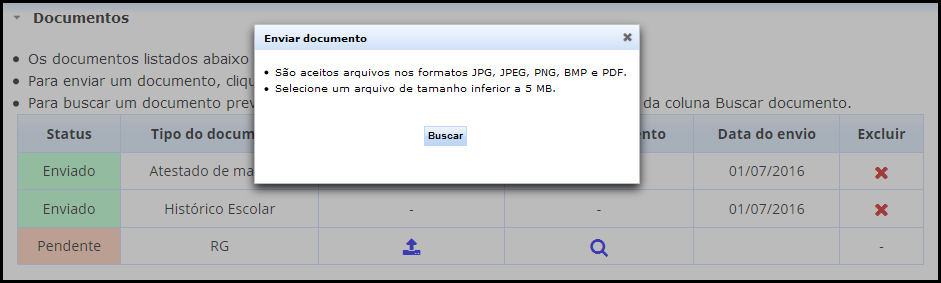
\includegraphics[width=1.0\textwidth]{/app/enviar_documento_desktop.png}
  \end{center}
  \fonte{Elaborada pelo autor.}
\end{figure}

No envio de documentos, uma caixa de diálogo modal informa os formatos aceitos pela aplicação e o tamanho máximo de cada arquivo. Ao clicar no botão \texttt{Buscar}, abre-se uma janela de busca de documentos nativa ao sistema operacional do computador do candidato para que este possa escolher o documento a ser enviado. Os documentos enviados são armazenados em um repositório e os identificadores dos arquivos são armazenados em um banco de dados (vide Figura~\ref{fig:uml_storage}).

Na busca de documentos, uma janela modal exibe uma lista de inscrições passadas nas quais esse mesmo tipo de documento foi utilizado. As colunas \texttt{Programa}, \texttt{Nível} e \texttt{Data do envio} auxiliam o candidato na escolha do documento a ser reutilizado na inscrição atual.

\begin{figure}[!ht]
  \caption{\label{fig:buscar_documento_desktop} Busca de documentos utilizados em inscrições passadas.}
  \begin{center}
    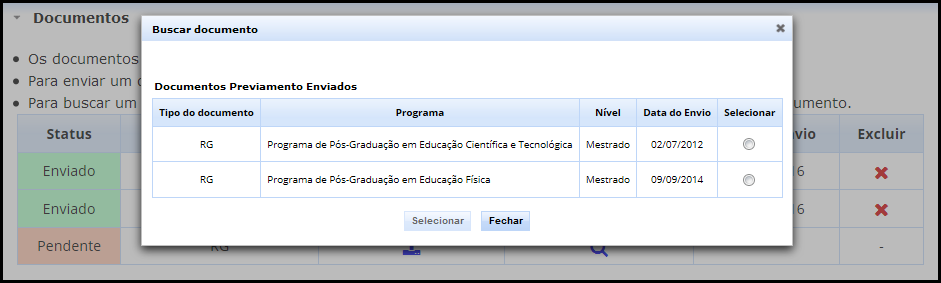
\includegraphics[width=1.0\textwidth]{/app/buscar_documento_desktop.png}
  \end{center}
  \fonte{Elaborada pelo autor.}
\end{figure}


Uma das preocupações que podem ser levantadas em relação ao envio de documentos é a quantidade de conexões simultâneas que o servidor onde está instalado o repositório de documentos suporta. Segundo dados obtidos na própria SeTIC, são possíveis sete conexões simultâneas ao repositório. Até o momento, o sistema atual não teve problemas relacionados à falta de conexões disponíveis. Embora o sistema em desenvolvimento vise atender a uma gama maior de secretarias, os processo seletivos dos diferentes programas costumam ter cronogramas diferentes, diminuindo a concorrência por conexões ao repositório.


% ---
\subsection{Verificação de erros e finalização de uma inscrição}\label{sec:validacao}
% ---

Pode-se verificar a existência de erros e o não-preenchimento de campos obrigatórios em qualquer momento durante o preenchimento do formulário através do botão \texttt{Verificar}\footnote{Salvo a situação em que o usuário está criando uma nova inscrição e ainda não salvou o formulário.}.
%
Na presença de tais erros, uma mensagem é exibida para o usuário e as abas que possuem campos não-preenchidos ou com erros são destacadas com ícone de exclamação, como pode ser visto na Figura~\ref{fig:verificacao_msg} para as abas \texttt{Dados Pessoais} e \texttt{Contato}.
%
\begin{figure}[!ht]
  \caption{\label{fig:verificacao_msg} Erros encontrados nas abas \texttt{Dados Pessoais} e \texttt{Contato}.}
  \begin{center}
    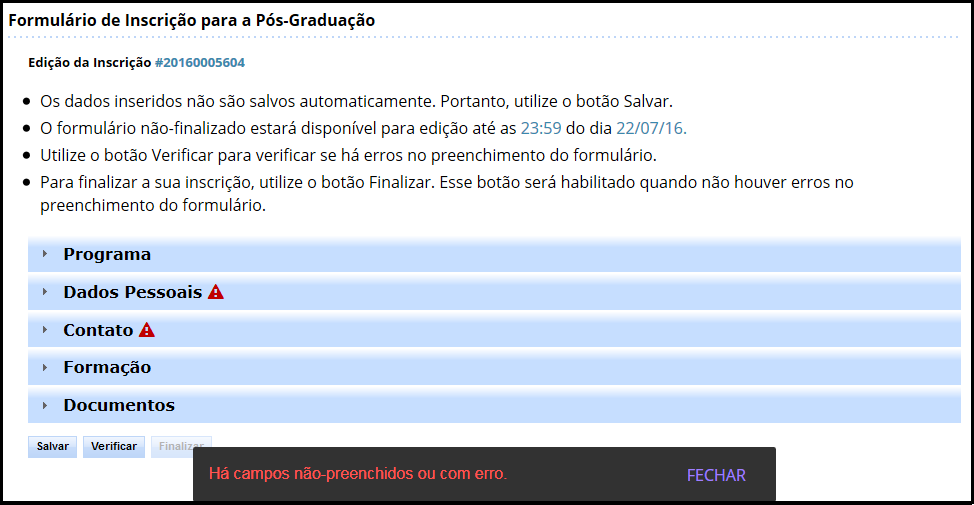
\includegraphics[width=1.0\textwidth]{/app/verificacao_msg_desktop.png}
  \end{center}
  \fonte{Elaborada pelo autor.}
\end{figure}

Ao abrir tais abas, os campos não-validados estão destacados na cor vermelha e com um ícone de exclamação ao lado de seus rótulos (vide Figura~\ref{fig:verificacao_aba}). Neste momento, tendo o usuário corrigido os erros ou não, se o formulário for salvo, os ícones de erro desaparecem.

Quando o formulário for verificado e não houver mais erros, uma mensagem de sucesso é exibida para o usuário (vide Figura~\ref{fig:verificacao_sucesso}), e o botão \texttt{Finalizar} é habilitado. Ao clicar no botão \texttt{Finalizar}, disponibiliza-se um comprovante de inscrição em formato PDF para o candidato e a edição da inscrição deixa de ser possível a partir deste momento. O documento é automaticamente descarregado no navegador e também enviado para o e-mail cadastrado pelo usuário no preenchimento do formulário. Um exemplo de comprovante é mostrado no Anexo~\ref{anexo:comprovante}.

\begin{figure}[!ht]
  \caption{\label{fig:verificacao_aba} Campos não-preenchidos da aba \texttt{Dados Pessoais}.}
  \begin{center}
    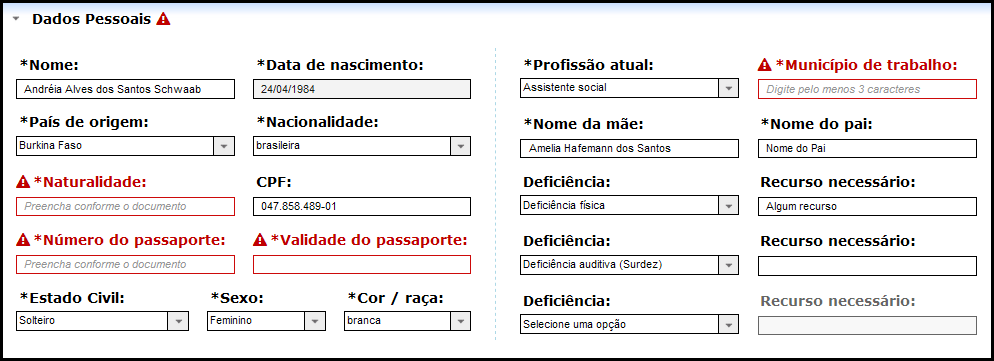
\includegraphics[width=1.0\textwidth]{/app/verificacao_aba_desktop.png}
  \end{center}
  \fonte{Elaborada pelo autor.}
\end{figure}


\begin{figure}[!ht]
  \caption{\label{fig:verificacao_sucesso} Formulário verificado e sem erros.}
  \begin{center}
    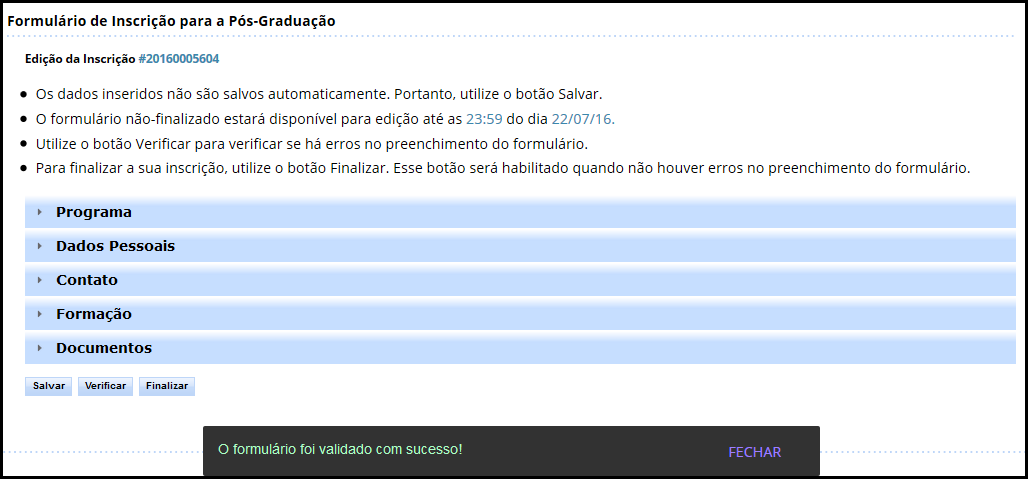
\includegraphics[width=1.0\textwidth]{/app/verificacao_sucesso_desktop.png}
  \end{center}
  \fonte{Elaborada pelo autor.}
\end{figure}

% ---
\subsection{Documentos enviados}\label{sec:documentos_enviados}
% ---

Todos os documentos enviados pelo candidato podem ser obtidos a partir da \emph{view documentos enviados}, a qual pode ser acessada através do item de menu \texttt{Documentos enviados}. O usuário pode baixar os documentos desejados clicando no ícone de \emph{download} da linha respectiva (vide Figura~\ref{fig:documentos_enviados}). Informações tais como número de inscrição, programa, nível, tipo de documento e data de envio também estão presentes para auxiliar o usuário a encontrar o documento desejado.


\begin{figure}[!ht]
  \caption{\label{fig:documentos_enviados} Lista de documentos enviados pelo candidato.}
  \begin{center}
    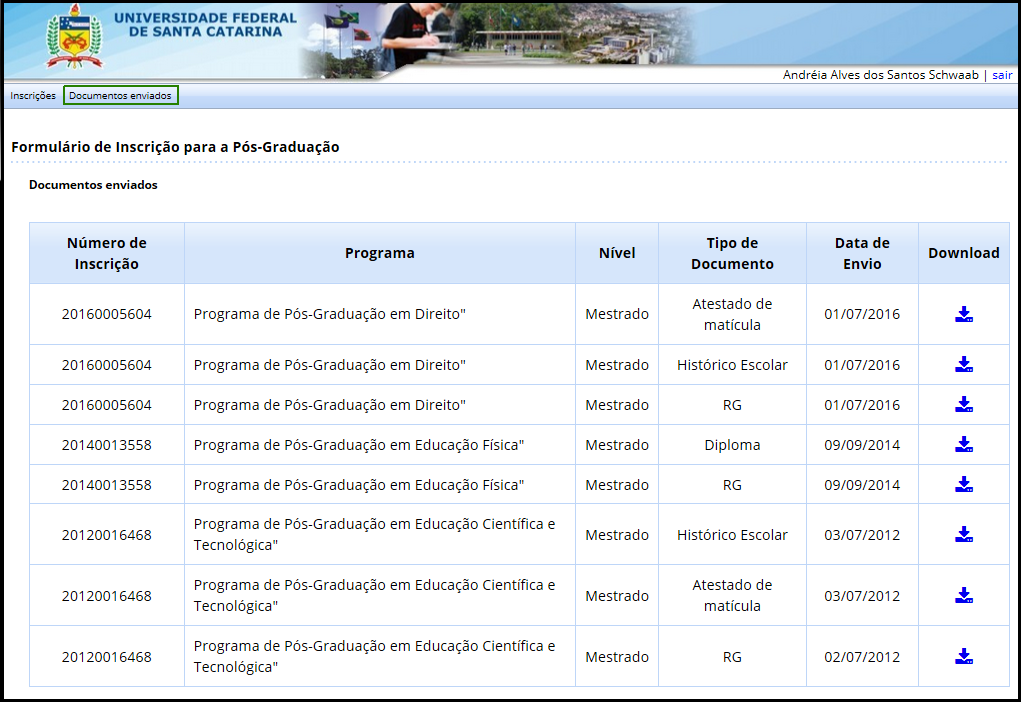
\includegraphics[width=1.0\textwidth]{/app/documentos_enviados_desktop.png}
  \end{center}
  \fonte{Elaborada pelo autor.}
\end{figure}



\chapter{Conclusões}
% ----------------------------------------------------------

O sistema de inscrição atual é utilizado por apenas alguns dos cursos de Pós-Graduação da UFSC. Alguns cursos utilizam seus próprios sistemas, dificultando a sua manutenibilidade e introduzindo duplicações de código e vulnerabilidades.

Torna-se imprescindível, portanto, o desenvolvimento de um novo sistema de inscrição unificado, que dê suporte a novas funcionalidades e que utilize as tecnologias atualmente em uso na SeTIC.

Ao longo deste projeto, diversas atividades previstas foram desenvolvidas, especificamente:
\begin{itemize}
  \item Levantamento das funcionalidades desejadas para o sistema através de entrevistas com o cliente (PROPG);
  \item Especificação dos requisitos funcionais e não-funcionais do sistema a partir destas funcionalidades;
  \item Definição da arquitetura do sistema a partir de diagramas feitos segundo as especificações da UML: diagrama de casos de uso, diagrama de visão geral de interação e diagramas de classes;
  \item Prototipação a partir do desenvolvimento de um conjunto de \emph{wireframes}.
  \item Adequação do Projeto Base para atender a estrutura definida;
  \item Implementação dos casos de uso discutidos na Seção~\ref{sec:funcionalidades}.
  \item Adaptação da interface do sistema para sua utilização em dispositivos móveis de forma responsiva.
\end{itemize}

O sistema desenvolvido está atualmente no estágio de homologação. A identificação de \emph{bugs}, as aprimorações e a adição de novas funcionalidades serão feitas por funcionários da SeTIC.

% ----------------------------------------------------------
\bibliography{referencias}

%\begin{thebibliography}{9}
%
%\bibitem{lamport94}
%  Leslie Lamport,
%  \emph{\LaTeX: a document preparation system},
%  Addison Wesley, Massachusetts,
%  2nd edition,
%  1994.
%\end{thebibliography}








\anexos

\chapter{Servlets}\label{anexo:servlets}
% ----------------------------------------------------------

\emph{Servlets} são classes Java que possuem métodos adequados a receber requisições e construir respostas às tais requisições dinamicamente. O trecho de código do Algoritmo~\ref{alg:servlet} representa um \texttt{HttpServlet} que atende a requisições HTTP do tipo GET através da sobrescrita do método \texttt{doGet()}. Os parâmetros \texttt{HttpServletRequest} e \texttt{HttpServletResponse} representam, respectivamente, a requisição feita pelo cliente e a resposta do servidor.
%
\begin{lstlisting}[language=Java, caption={Um \emph{servlet} que imprime ``\emph{Hello World}''.}, label={alg:servlet}]
import java.io.*;
import javax.servlet.*;
import javax.servlet.http.*;

public class HelloWorld extends HttpServlet {
  public void doGet(HttpServletRequest req,
                    HttpServletResponse res)
      throws ServletException, IOException {
    res.setContentType("text/html");
    PrintWriter out = res.getWriter();
    out.println("<html>");
    out.println("<head><title>Hello World</title></head>");
    out.println("<body>");
    out.println("<big>Hello World</big>");
    out.println("</body></html>");
  }
}
\end{lstlisting}
\fonte{adaptado de \citeonline{javaservlet}}

Um \emph{servlet} HTTP pode, além do método \texttt{doGet()}, sobreescrever outros métodos, tais como \texttt{doPut()}, \texttt{doDelete()}, etc, que representam requisições HTTP do tipo PUT, DELETE, etc, respectivamente.



\chapter{Relacionamentos JPA}\label{anexo:jpa}
% ----------------------------------------------------------


\section{Relacionamento \texttt{@OneToOne}}
Apenas uma instância da entidade fonte\footnote{A entidade na qual se está fazendo a anotação.} pode referenciar a mesma instância da entidade alvo. Em termos do banco de dados, isso implica na existência de uma restrição de unicidade na coluna da chave estrangeira da tabela fonte. Ainda, o JPA espera que o nome dessa coluna seja igual ao nome do atributo da entidade fonte seguido de um \emph{underscore} e do nome da coluna da chave primária da tabela alvo. Caso esse não seja o caso, então deve-se fornecer o nome da coluna na anotação \texttt{@JoinColumn}.

Para ilustrar essa situação, considere as tabelas ilustradas na Figura~\ref{fig:jpa_onetoone}. O mapeamento feito pelo JPA espera que a coluna com a chave estrangeira a ser utilizada seja chamada de \texttt{PARKINGSPACE\_ID}, porém essa coluna chama-se \texttt{PSPACE\_ID}. Neste caso, utiliza-se a anotação \texttt{@JoinColumn(name = ``PSPACE\_ID'')}, conforme Algoritmo~\ref{alg:entity_employee}.



\begin{figure}[!ht]
  \caption{\label{fig:jpa_onetoone} Tabelas EMPLOYEE e PARKING\_SPACE.}
  \begin{center}
    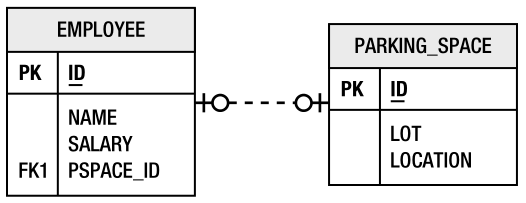
\includegraphics[width=0.75\textwidth]{/jpa/one_to_one_table.png}
  \end{center}
  \fonte{Retirado de \citeonline{keith2013}.}
\end{figure}

É interessante notar que o campo \texttt{name} não possui nenhuma anotação relacionada à sua persistência. Isso se deve ao fato de existir uma coluna de mesmo nome na tabela \texttt{EMPLOYEE}.

\begin{lstlisting}[caption={Classe Employee e seus relacionamentos.}, label={alg:entity_employee}]
@Entity
public class Employee {

  @Id private long id;
  
  @OneToOne
  @JoinColumn(name = "PSPACE_ID")
  private ParkingSpace parkingSpace;
  // ...
}
\end{lstlisting}
\fonte{Adaptado de \citeonline{keith2013}.}


Quando a entidade alvo do relacionamento também possuir uma referência à entidade fonte, tem-se então um relacionamento bidirecional, em que uma das entidades é dita ser a \emph{dona} do relacionamento por conter a coluna com a chave estrangeira da outra entidade\footnote{A escolha de qual das tabelas deverá conter a chave estrangeira da outra tabela é uma decisão de modelagem do banco de dados.}. Nessa situação, a anotação \texttt{@JoinColumn} da entidade que \emph{não} é a dona do relacionamento recebe o elemento \texttt{mappedBy = "X"}, onde X refere-se ao nome do campo da entidade que é dona do relacionamento, como pode ser visto no Algoritmo~\ref{alg:entity_employee_bi}.

\begin{lstlisting}[caption={Classe ParkingSpace e seus relacionamentos.}, label={alg:entity_employee_bi}]
@Entity
public class ParkingSpace {
  
  @Id private long id;
  private String location;

  @OneToOne(mappedBy = "parkingSpace")
  private Employee employee;
  // ...
}
\end{lstlisting}
\fonte{Adaptado de \citeonline{keith2013}.}%

\section{Relacionamento \texttt{@OneToMany}}

Este tipo de relacionamento ocorre quando uma entidade está associada a uma coleção de entidades. Considere as tabelas \texttt{EMPLOYEE} e \texttt{DEPARTMENT} ilustradas na Figura~\ref{fig:jpa_onetomany}. O relacionamento \emph{um para muitos} feito em UML pode ser visto em (b).

\begin{figure}[!ht]
  \caption{\label{fig:jpa_onetomany} Tabelas \texttt{EMPLOYEE} e \texttt{DEPARTMENT} em (a) e seu relacionamento em (b).}
  \begin{center}
    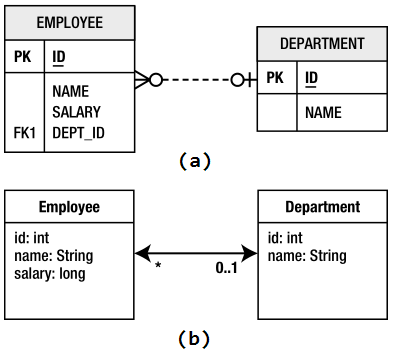
\includegraphics[width=0.75\textwidth]{/jpa/one_to_many.png}
  \end{center}
  \fonte{Adaptado de \citeonline{keith2013}.}
\end{figure}


É importante notar que esse relacionamento implica em um relacionamento \emph{muitos para um} quando analisado a partir da tabela \texttt{EMPLOYEE} e, portanto, é um relacionamento naturalmente bidirecional. Daí que uma das entidades fará o papel de dona do relacionamento, conforme discutido anteriormente no caso do relacionamento \emph{um para um} bidirecional. Devido ao fato de não existir uma maneira escalonável de guardar inúmeras chaves em uma única linha de uma tabela, a entidade dona do relacionamento nessa situação deve ser a que estiver no lado ``muitos''. Nesse caso, a entidade dona é, portanto, a \texttt{EMPLOYEE} e nela estarão as chaves estrangeiras para as linhas da tabela \texttt{DEPARTMENT}. Por sua vez, isso implica na adição do elemento \texttt{mappedBy} na anotação \texttt{@JoinColumn} dessa última entidade, conforme Algoritmo~\ref{alg:entity_dept}.

\begin{lstlisting}[caption={Classe Department e seus relacionamentos.}, label={alg:entity_dept}]
@Entity
  public class Department {

  @Id
  private long id;
  private String name;

  @OneToMany(mappedBy = "department")
  private Collection<Employee> employees;
  // ...
}
\end{lstlisting}
\fonte{Adaptado de \citeonline{keith2013}.}%

Mais uma vez, devido à utilização de um nome de coluna diferente do valor padrão esperado para esse relacionamento, utiliza-se o elemento \texttt{name} na anotação \texttt{@JoinColumn} da entidade Employee (vide Algoritmo~\ref{alg:entity_employee2}).

\begin{lstlisting}[caption={Classe Employee e seus relacionamentos.}, label={alg:entity_employee2}]
@Entity
public class Employee {

  @Id
  private long id;

  @ManyToOne
  @JoinColumn(name = "DEPT_ID")
  private Department department;
  // ...
}
\end{lstlisting}
\fonte{Adaptado de \citeonline{keith2013}.}%


\section{Relacionamento \texttt{@ManyToMany}}

O último tipo de relacionamento entre entidades apresentado é chamado de \emph{muitos para muitos}. Esse relacionamento ocorre quando uma ou mais entidades fonte estão associadas a uma coleção de entidades alvo, e estas entidades alvo estão associadas a uma coleção de entidades fonte. A representação dessa situação em UML pode ser vista no item (b) da Figura~\ref{fig:jpa_manytomany} para as entidades Employee e Project.

Considere agora as tabelas ilustradas no item (a) da Figura~\ref{fig:jpa_manytomany}. Uma linha de \texttt{EMPLOYEE} pode estar associada a diversas linhas de \texttt{PROJECT} e vice-versa. A existência da tabela \texttt{EMP\_PROJ} justifica-se por não ser escalável guardar as chaves estrangeiras em cada linha de \emph{ambas} as tabelas. Nesse caso, \texttt{EMP\_PROJ} possui apenas duas colunas e estas guardam as chaves estrangeiras de cada uma das tabelas. Portanto, \texttt{EMPLOYEE} não possui uma coluna com as chaves estrageiras de \texttt{PROJECT} e vice-versa \cite{keith2013}.

\begin{figure}[!ht]
  \caption{\label{fig:jpa_manytomany} Tabelas \texttt{EMPLOYEE},  \texttt{EMP\_PROJ} e \texttt{PROJECT} em (a) e seu relacionamento em (b).}
  \begin{center}
    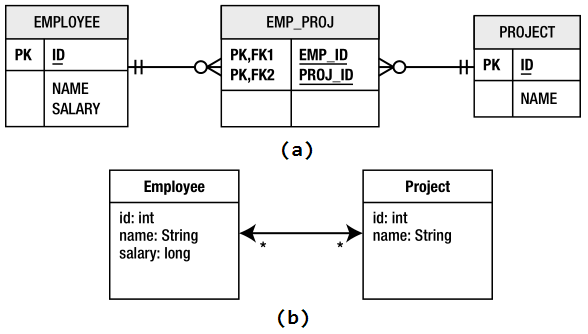
\includegraphics[width=1.0\textwidth]{/jpa/many_to_many.png}
  \end{center}
  \fonte{Adaptado de \citeonline{keith2013}.}
\end{figure}

Se ambas as tabelas \texttt{EMPLOYEE} e \texttt{PROJECT} não possuem uma coluna de chaves estrangeiras, quem é a entidade dona do relacionamento? A resposta é: tanto faz, desde que essa decisão seja indicada ao JPA. As entidades Employee e Project resultantes do mapeamento podem ser vistas no Algoritmo~\ref{alg:entity_employee_project}. Evidencia-se o uso da anotação \texttt{joinColumns}, indicando a entidade dona do relacionamento.


\begin{lstlisting}[caption={Classes Employee e Project.}, label={alg:entity_employee_project}]
@Entity
public class Employee {
  @Id
  private long id;
  private String name;
  @ManyToMany
  @JoinTable(name="EMP_PROJ",
      joinColumns=@JoinColumn(name="EMP_ID"),
      inverseJoinColumns=@JoinColumn(name="PROJ_ID"))
  private Collection<Project> projects;
  // ...
}

@Entity
public class Project {
  @Id
  private long id;
  private String name;
  @ManyToMany(mappedBy="projects")
  private Collection<Employee> employees;
  // ...
}
\end{lstlisting}
\fonte{Adaptado de \citeonline{keith2013}.}%



\chapter{RUP: melhores práticas}\label{anexo:rup}
% ----------------------------------------------------------

Com o intuito de minimizar as falhas e aumentar a produtividade no desenvolvimento de software, seis idéias, conhecidas por \emph{seis melhores práticas}, são descritas no RUP. São chamadas de \emph{melhores} práticas por serem comumente observadas em organizações bem sucedidas.

\begin{enumerate}
\item \textbf{Desenvolver software iterativamente} --- Identificar o problema por completo, desenvolver uma solução, construir o software e testar o produto, é uma abordagem muito arriscada de se seguir de forma sequencial, dados os sistemas de software complexos dos dias de hoje. A adoção de uma abordagem iterativa permite um entendimento do problema de forma gradativa através de múltiplas iterações. Como cada iteração resulta em um \emph{release} executável, o time de desenvolvimento permanece sempre focado em alcançar as metas de cada iteração, além de possibilitar um melhor controle do cronograma das atividades. Ainda, os requisitos de maior risco são abordados no início de cada estágio, reduzindo, assim, o perfil de risco do projeto.

\item \textbf{Gerenciar requisitos} --- O RUP descreve como elicitar, organizar e documentar as funcionalidades e restrições do sistema, bem como fazer o monitoramento das decisões adotadas ao longo do desenvolvimento do projeto. Além disso, a utilização de \emph{casos de uso} como forma de capturar os requisitos funcionais e direcionar o design, a implementação e o teste de software, aumenta a probabilidade de que o sistema irá satisfazer as necessidades do usuário final.

\item \textbf{Usar arquiteturas baseadas em componentes} --- O desenvolvimento de sistemas altamente complexos de forma monolítica aumenta substancialmente os riscos envolvidos no projeto. A utilização de módulos ou subsistemas que satisfazem funções específicas permite o reuso de código e a realização de testes antes da sua integração.

\item \textbf{Modelar o software visualmente} --- A utilização de diagramas para a modelagem de atores, componentes e suas interações permite a visualização da estrutura e comportamento dos diversos componentes do sistema de forma abstrata. Segundo o RUP, a UML é considerada o alicerce para a modelagem visual.

\item \textbf{Verificar a qualidade do software} --- A aceitação das aplicações de software é drasticamente inibida por baixo desempenho e confiabilidade. A avaliação da qualidade do software é feita através de testes de funcionalidade e desempenho da aplicação e do sistema, com base nos requisitos especificados.

\item \textbf{Controlar as mudanças feitas no software} --- A utilização de uma sistema de controle de mudanças é indispensável em um ambiente em que mudanças são inevitáveis. A identificação de quando uma mudança ocorreu e quem a realizou é muito útil para a sincronização e estabelecimento de áreas de trabalho seguras para os desenvolvedores.
\end{enumerate}



\chapter{Exemplificação para dispositivos móveis}\label{anexo:mobile}
% ----------------------------------------------------------

\begin{figure}[!ht]
  \caption{\label{fig:mobile_index_programas} À esquerda: página inicial do sistema, a partir da qual pode-se obter a lista de programas disponíveis para inscrição e iniciar a sessão. À direita: lista de programas disponíveis. }
  \begin{center}
    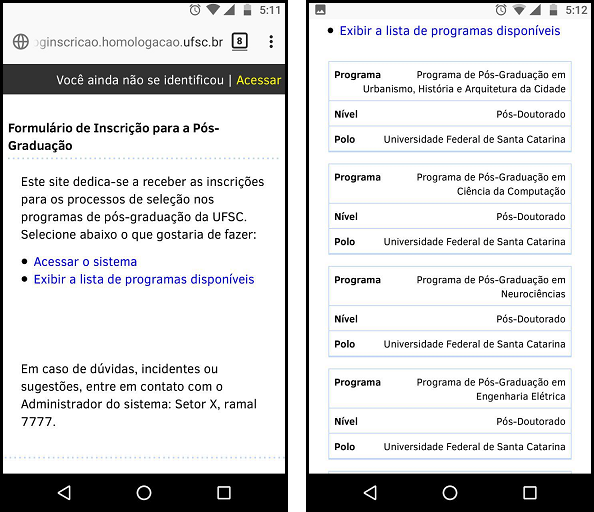
\includegraphics[width=1.0\textwidth]{/app/mobile_index_programas.png}
  \end{center}
  \fonte{Elaborada pelo autor.}
\end{figure}


\begin{figure}[!ht]
  \caption{\label{fig:mobile_inscricoes} À esquerda: \emph{view} inscrições após a autenticação. À direita: detalhe para os dois tipos de inscrição. As linhas de uma tabela comum se transformam em pequenos blocos cujo número de linhas é igual ao número de colunas da tabela no modo \emph{desktop}.}
  \begin{center}
    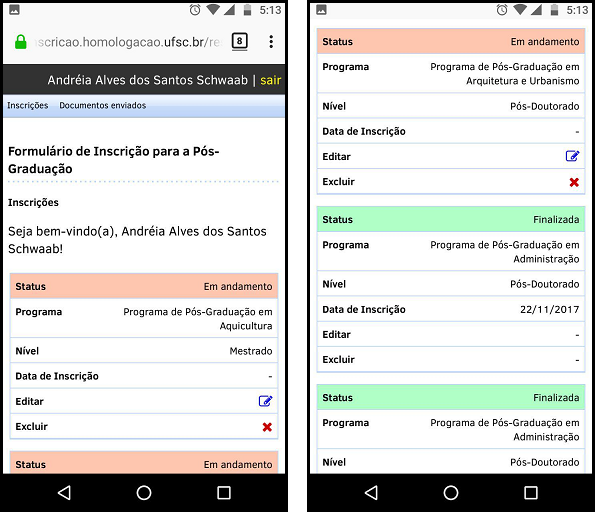
\includegraphics[width=1.0\textwidth]{/app/mobile_inscricoes.png}
  \end{center}
  \fonte{Elaborada pelo autor.}
\end{figure}

\begin{figure}[!ht]
  \caption{\label{fig:mobile_criar_inscricao} À esquerda: criação de uma nova inscrição. Em detalhe: aba \texttt{Programa} vazia. À direita: mensagem de importar dados da última inscrição realizada.}
  \begin{center}
    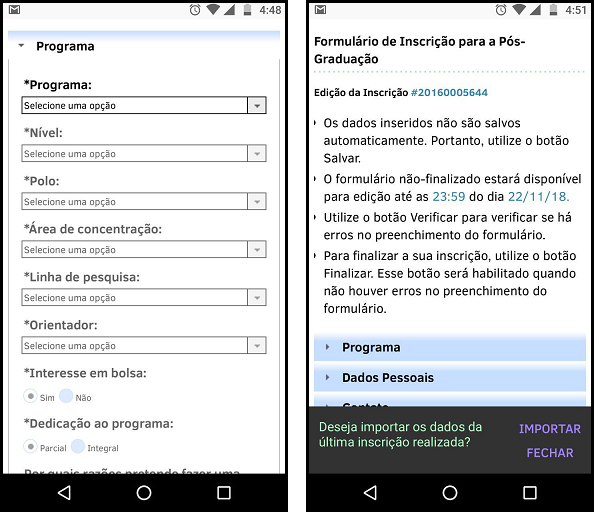
\includegraphics[width=1.0\textwidth]{/app/mobile_criar_inscricao.png}
  \end{center}
  \fonte{Elaborada pelo autor.}
\end{figure}

\begin{figure}[!ht]
  \caption{\label{fig:mobile_dados_pessoais_contato} Preenchimento do formulário com dados fictícios. À esquerda: campos da aba \texttt{Dados Pessoais}. À direita: campos da aba \texttt{Contato}.}
  \begin{center}
    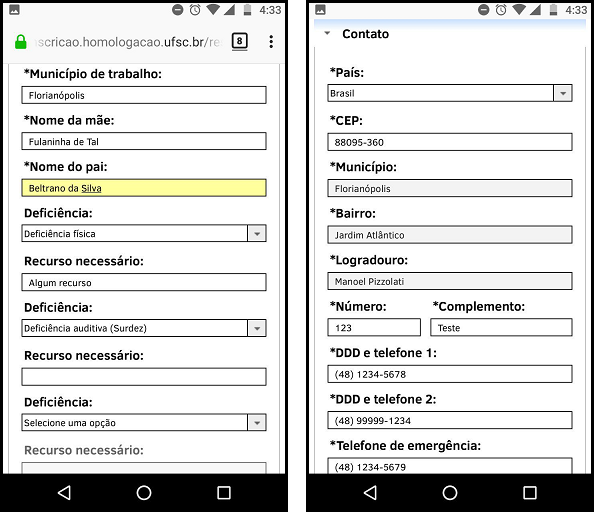
\includegraphics[width=1.0\textwidth]{/app/mobile_dados_pessoais_contato.png}
  \end{center}
  \fonte{Elaborada pelo autor.}
\end{figure}

\begin{figure}[!ht]
  \caption{\label{fig:mobile_formacao} Preenchimento do formulário com dados fictícios. À esquerda: aba \texttt{Formação} com um curso de formação em andamento. À direita: caixa de diálogo modal de inclusão de um curso de formação.}
  \begin{center}
    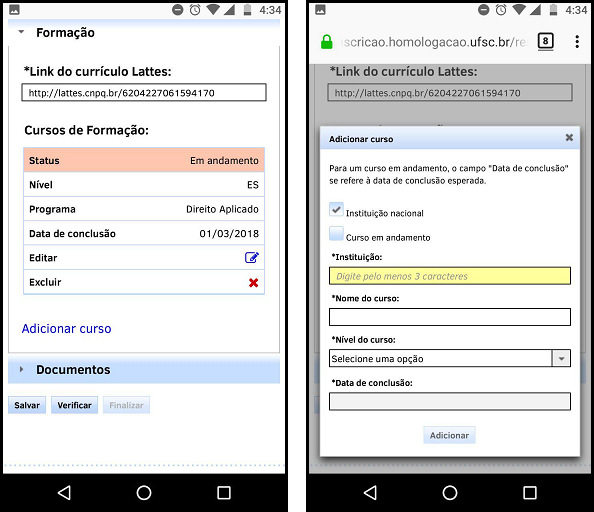
\includegraphics[width=1.0\textwidth]{/app/mobile_formacao.png}
  \end{center}
  \fonte{Elaborada pelo autor.}
\end{figure}

\begin{figure}[!ht]
  \caption{\label{fig:mobile_documentos} À esquerda: mensagens informativas da aba \texttt{Documentos}. À direita: caixa de diálogo modal para a reutilização de documentos enviados em inscrições passadas mostrando dois documentos do tipo RG.}
  \begin{center}
    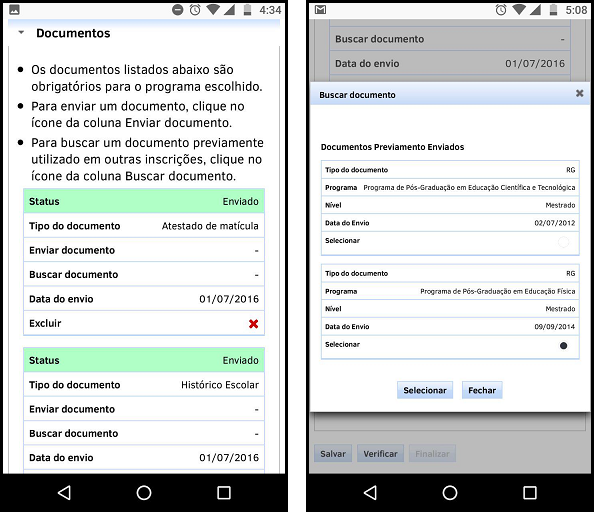
\includegraphics[width=1.0\textwidth]{/app/mobile_documentos.png}
  \end{center}
  \fonte{Elaborada pelo autor.}
\end{figure}


\begin{figure}[!ht]
  \caption{\label{fig:mobile_verificacao_erros} À esquerda: erros encontrados no preenchimento do formulário. À direita: destaque para o campo não-preenchido na aba \texttt{Dados pessoais}.}
  \begin{center}
    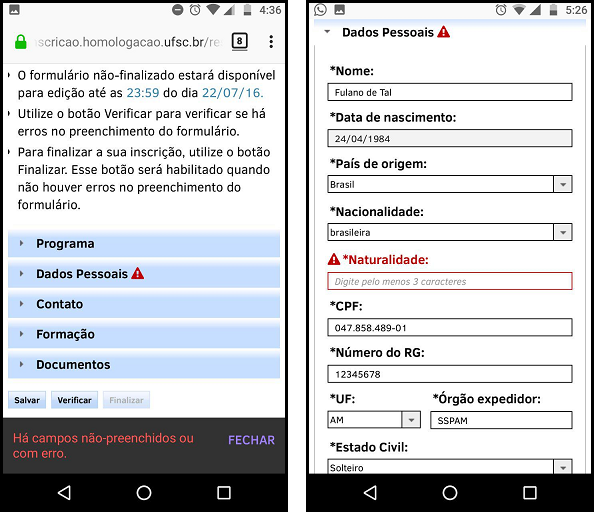
\includegraphics[width=1.0\textwidth]{/app/mobile_verificacao_erros.png}
  \end{center}
  \fonte{Elaborada pelo autor.}
\end{figure}

\begin{figure}[!ht]
  \caption{\label{fig:mobile_verificacao_sucesso_documentos_enviados} À esquerda: formulário verificado e sem erros. Botão \texttt{Finalizar} habilitado. À direita: tela de documentos enviados pelo candidato.}
  \begin{center}
    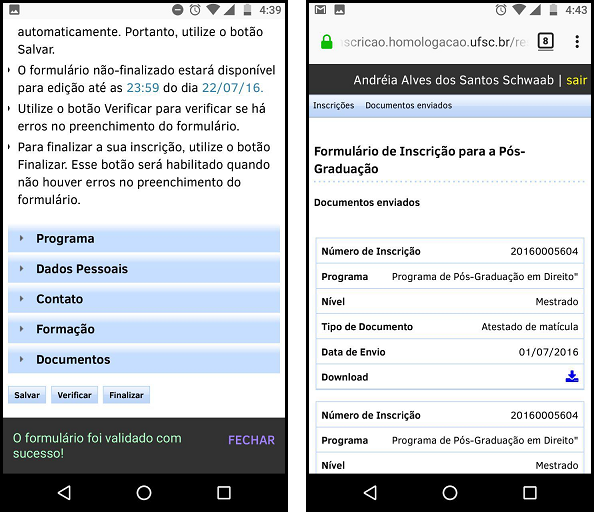
\includegraphics[width=1.0\textwidth]{/app/mobile_verificacao_sucesso_documentos_enviados.png}
  \end{center}
  \fonte{Elaborada pelo autor.}
\end{figure}



\chapter{Exemplo de comprovante de inscrição}\label{anexo:comprovante}
% ----------------------------------------------------------
\noindent
\fbox{
\includegraphics[width=1.0\textwidth]{comprovante.pdf}}

\end{document}

% EXEMPLO DE TABELA DO IBGE
%
%\begin{table}[!htb]
%  \IBGEtab{%
%    \caption{Um Exemplo de tabela alinhada que pode ser longa ou curta, conforme padrão IBGE.}%
%    \label{tabela-ibge}
%  }{%
%    \begin{tabular}{ccc}
%      \toprule
%      Nome & Nascimento & Documento \\
%      \midrule \midrule
%      Maria da Silva & 11/11/1111 & 111.111.111-11 \\
%      \bottomrule
%    \end{tabular}%
%  }{%
%    \fonte{Produzido pelos autores}%
%    \nota{Esta é uma nota, que diz que os dados são baseados na regressão linear.}%
%    \nota[Anotações]{Uma anotação adicional, seguida de várias outras.}%
%  }
%\end{table}